% !TEX root = ../thesis.tex
%
\chapter{Proponowane algorytmy}
\label{sec:proponowane_algorytmy}

Niniejszy rozdział szczegółowo opisuje kolejne kroki rozwiązania problemu dokładnie przestawionego w sekcji \ref{sec:wstep:opis_problemu}. Sekcja \ref{sec:proponowane_algorytmy:wiedza_dziedzinowa} opisuje wiedzę dziedzinową na temat danych wejściowych (kafelków). Następnie sekcje od \ref{sec:proponowane_algorytmy:sift} do \ref{sec:proponowane_algorytmy:laczenie_kafelkow} opisują zasadę działania poszczególnych metod w kolejności zgodnej z ich wykonywaniem w programie.

\section{Wiedza dziedzinowa}
\label{sec:proponowane_algorytmy:wiedza_dziedzinowa}

Wiedza dziedzinowa określa zbiór informacji związanych z problemem i danymi wejściowymi. Dokładne zdefiniowanie oraz analiza wiedzy dziedzinowej prowadzi do ułatwienia problemu oraz lepszych rezultatów. W przypadku problemu niniejszej pracy danymi wejściowymi do stworzenia mozaiki są angiograficzne obrazy OCT (kafelki). Są to monochromatyczne obrazy o rozmiarze 240 na 240 pikseli. Wraz z obrazami do programu dostarczane są jeszcze dwie informacje:

\begin{itemize}
\item Względna pozycja kafelków względem siebie zapisana w nazwie obrazu. Lokalizacja jest podana za pomocą współrzędnych x i y układu kartezjańskiego.
\item Szacowany obszar nałożenia kafelków na siebie wyrażony w procentach szerokości obrazu.
\end{itemize}

Na rysunku \ref{fig:proponowane_algorytmy:example} jest przedstawiony przykładowy zbiór kafelków przeznaczony do stworzenia jednej mozaiki wraz z dostarczoną wiedzą dziedzinową.

\begin{figure}[H]
  \centering
  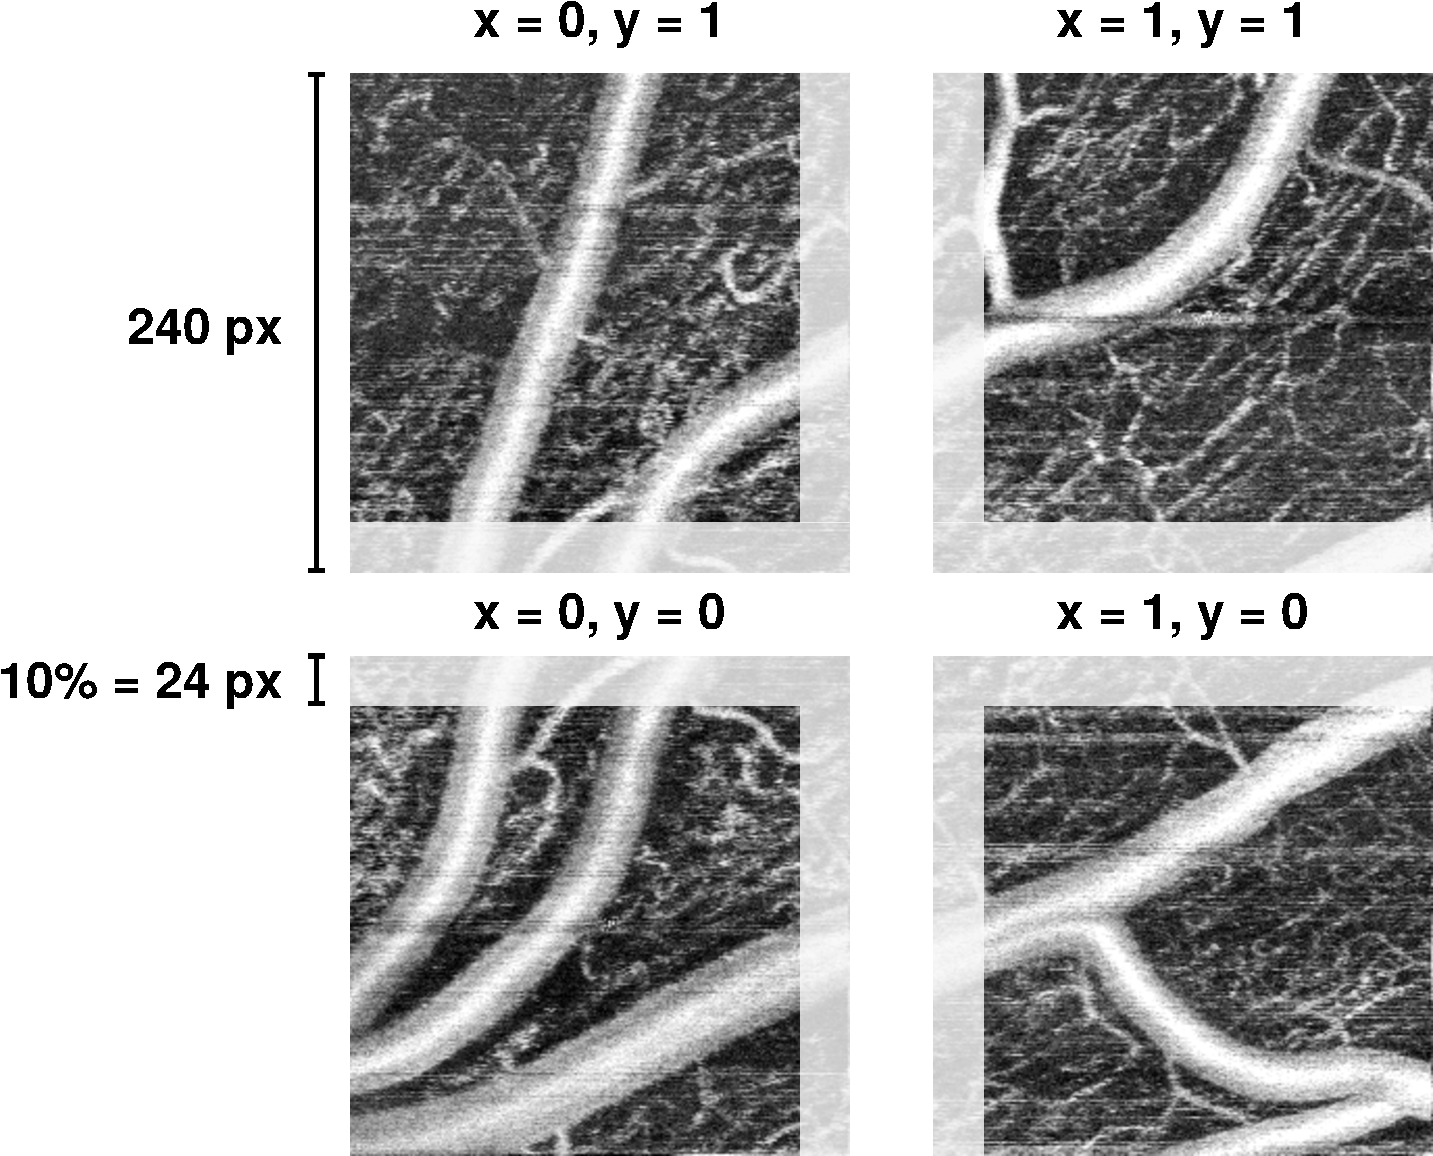
\includegraphics[width=\textwidth]{gfx/example}
  \caption{Cztery kafelki rozmieszone zgodnie z ich pozycją w docelowej mozaice. Na każdym obrazie białym przeźroczystym prostokątem zaznaczony jest oszacowany obszar nałożenia sąsiadujących kafelków.}
  \label{fig:proponowane_algorytmy:example}
\end{figure}

Informacje dostarczone wraz z kafelkami mają istotny wpływ na działanie algorytmu. Położenie kafelków informuje algorytm, który kafelek należy dopasowywać z którym (sekcja \ref{sec:proponowane_algorytmy:filtrowanie}), a szacowany obszar nałożenia określa obszar ekstrahowania cech (sekcja \ref{sec:proponowane_algorytmy:sift}). Bez tych informacji stworzenie mozaiki byłoby o wiele bardziej skomplikowane.

\section{Rejestracja kafelków z wykorzystaniem cech}
\label{sec:proponowane_algorytmy:cechy}

Ekstrakcja cech jest pierwszym krokiem tworzenia mozaiki. W niniejszej sekcji najpierw jest wyjaśniony wybrany algorytm do ekstrakcji cech oraz sposób jego użycia w programie (sekcja \ref{sec:proponowane_algorytmy:sift}). Następnie przedstawiony jest proces dopasowania wyekstrahowanych cech do siebie (sekcja \ref{sec:proponowane_algorytmy:dopasowanie}), a na koniec tej sekcji wyjaśnione jest filtrowanie znalezionych dopasowań (sekcja \ref{sec:proponowane_algorytmy:filtrowanie}).

\subsection{Algorytm SIFT}
\label{sec:proponowane_algorytmy:sift}

\textbf{SIFT} (ang. \textit{scale-invariant feature transform}) to algorytm służący do wykrycia i opisania cech w obrazie. Metodę opublikowano w 1999 roku przez David Lowe \cite{Lowe:2004:DIF:993451.996342}. Dzięki umiejętności wyekstrahowania cech, które są niewrażliwe na rotacje, skalowanie, lokalizacje i przekształcenie afiniczne obrazu SIFT jest stosowany w wielu aplikacjach (np. lokalizacja robota \cite{conf/icra/2001}, czy rozpoznawanie zachowań człowieka \cite{Laptev:2007:LVM:1314710.1314906}).

Działanie algorytmu można podzielić na 6 kroków:

\subsubsection{1. Reprezentacja obszaru za pomocą przestrzeni \textit{scale-space}}
\label{sec:proponowane_algorytmy:scale_space}

Algorytm rozpoczyna swoją pracę tworząc przestrzeń \textit{scale-space} obszaru obrazu służący do ekstrakcji cech. \textit{Scale-space} generuje się poprzez kilkakrotne użycie filtru Gaussa z różną siłą na docelowym obszarze. Następnie oryginalny obraz próbkujemy zmniejszając jego wielkość dwukrotnie i powtarzamy proces użycia filtru Gaussa. Obrazy o tej samej wielkości tworzą oktawę. Na rysunku \ref{fig:proponowane_algorytmy:scale_space_fig} pokazana jest przestrzeń \textit{scale-space} dla przykładowego obrazu.

\begin{figure}[H]
  \centering
  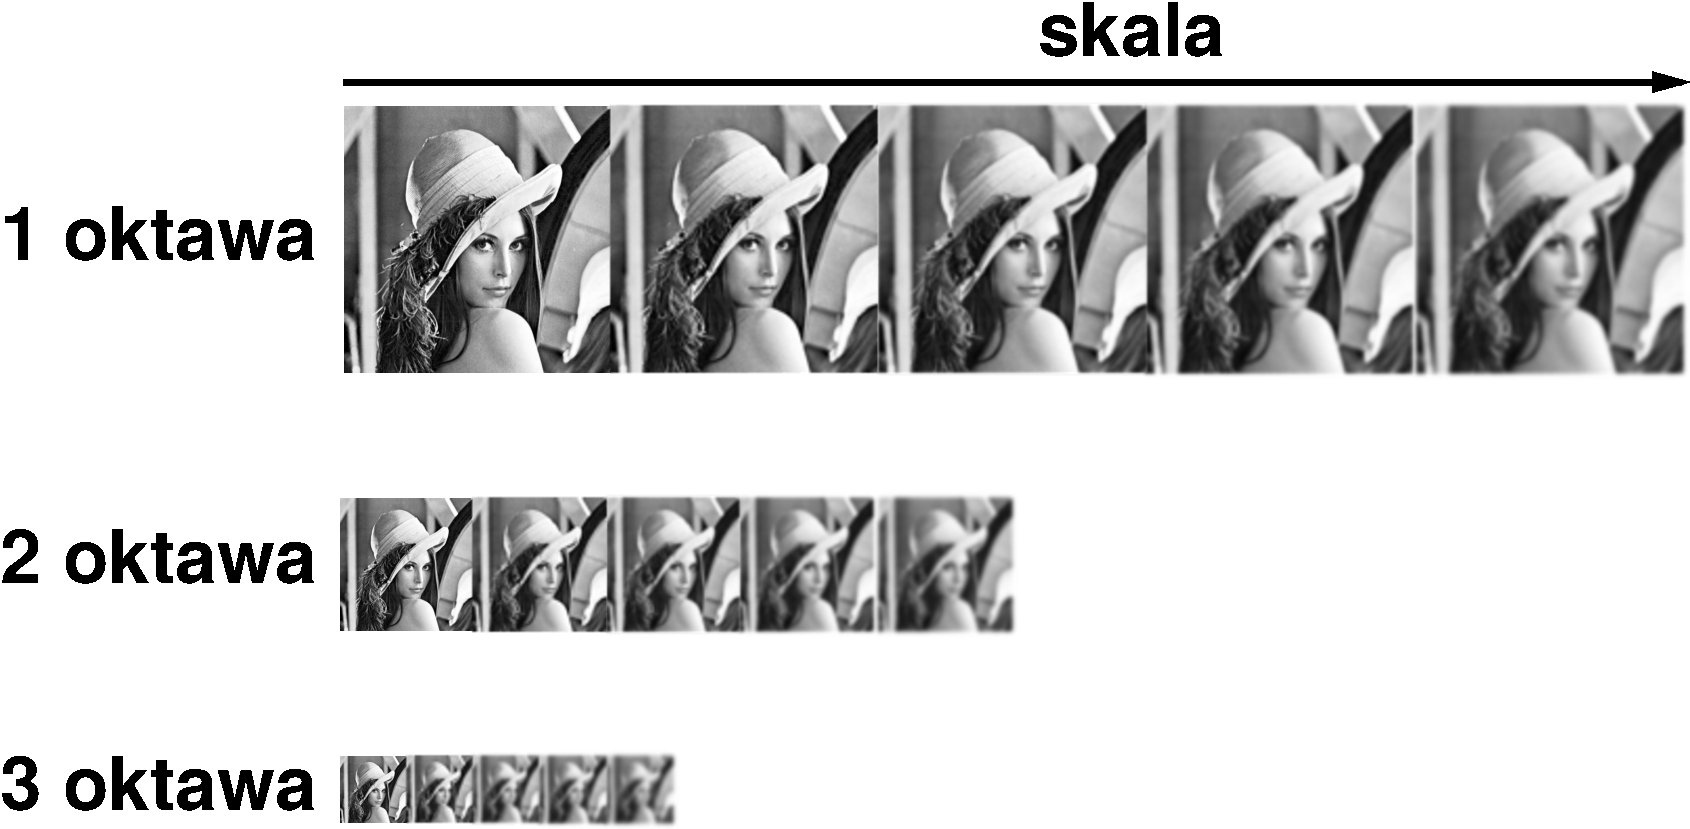
\includegraphics[width=10cm]{gfx/scale_space}
  \caption{Przestrzeń \textit{scale-space} dla przykładowego obrazu. Skala rośnie wraz z siłą filtru Gaussa. Obrazy tej samej wielkości tworzą oktawę.}
  \label{fig:proponowane_algorytmy:scale_space_fig}
\end{figure}

Autor algorytmu SIFT zalecana użycie czterech oktaw i pięciu poziomów siły filtru Gaussa.

\subsubsection{2. Obliczenie \textit{difference of Gaussians}}
\label{sec:proponowane_algorytmy:difference}

Charakterystycznymi punktami obrazu są krawędzie i rogi. Są to miejsca najlepiej nadające się na znalezienie cech. Operacja \textit{laplacian of Gaussian, LoG} świetnie sobie radzi w wykrywaniu krawędzi i rogów w obrazie. Polega ona na wyeliminowaniu szumu poprzez zaaplikowanie filtru Gaussa, a następnie obliczenie drugiej pochodnej. Na rysunku \ref{fig:proponowane_algorytmy:gauss} przedstawione jest działanie LoG na jednowymiarowym fragmencie obrazu.

\begin{figure}[H]
  \centering
  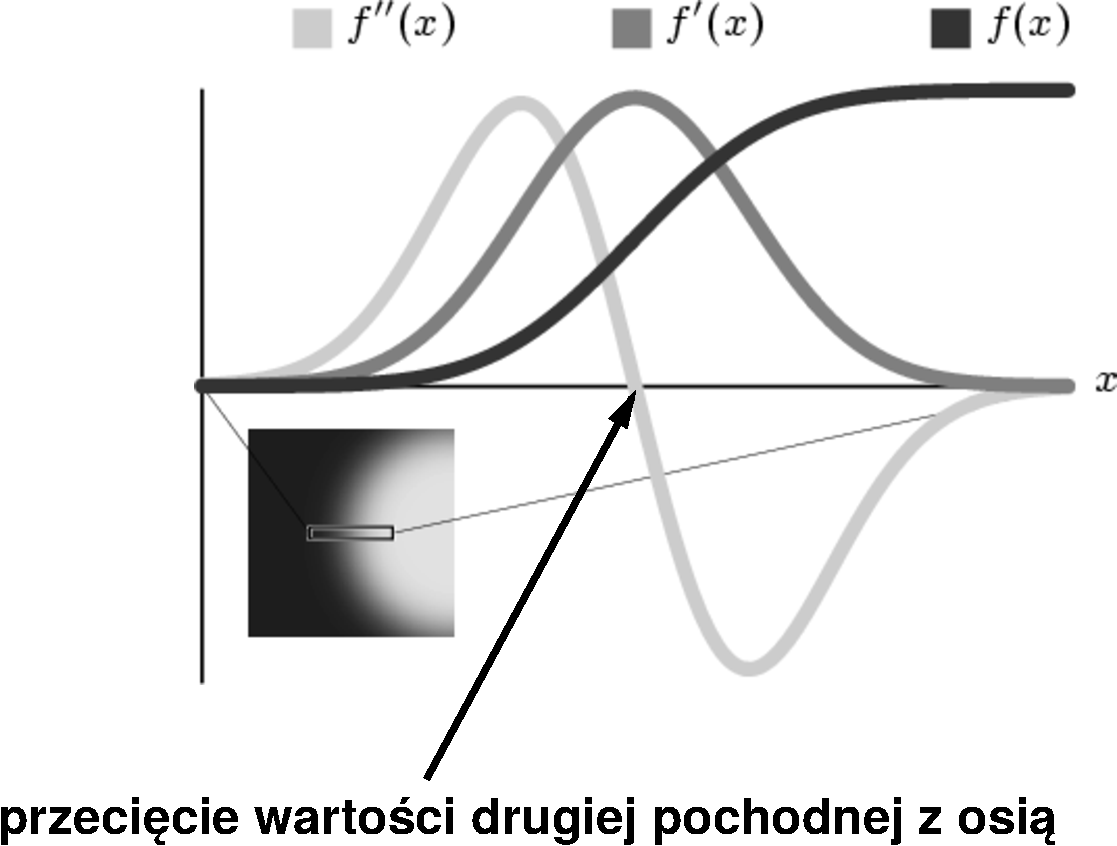
\includegraphics[width=8cm]{gfx/gauss}
  \caption{Przykład wykrycia krawędzi przez LoG. Czarny wykres przedstawia jednowymiarowy sygnał z obrazu. Miejsce przecięcia się z osią drugiej pochodnej tzw. \textit{zero-crossing} wskazuje miejsce krawędzi w oryginalnym obrazie.}
  \label{fig:proponowane_algorytmy:gauss}
\end{figure}

Obliczenie drugiej pochodnej całego obrazu jest natomiast kosztownym procesem. SIFT implementuje operację \textit{difference of Gaussians, DoG} dającą niemal identyczny wynik do LoG, ale jest o wiele szybsza. DoG polega na odjęciu dwóch kolejnych obrazów z tej samej oktawy. Rysunek \ref{fig:proponowane_algorytmy:dog} przedstawia operację DoG. DoG jest obliczane dla każdej pary w każdej oktawie.

\begin{figure}[htb]
  \centering
  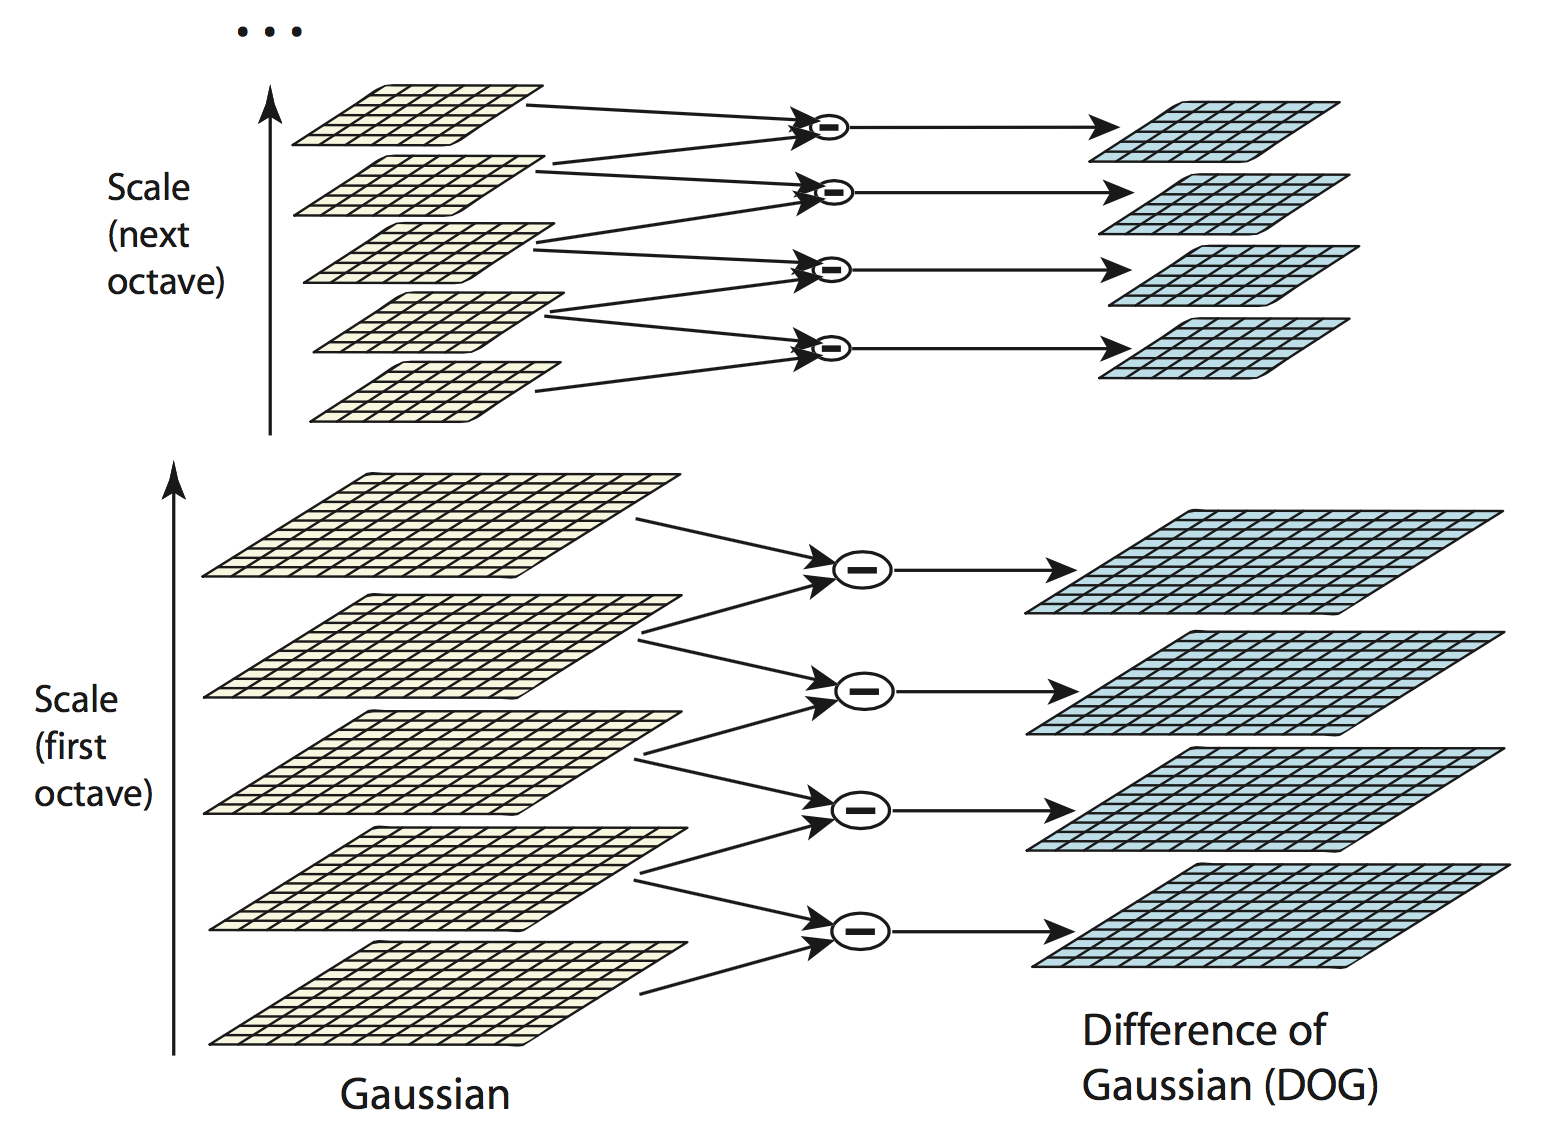
\includegraphics[width=10cm]{gfx/dog}
  \caption{\cite{Lowe:2004:DIF:993451.996342} Poprzez proces odjęcia kolejnych zdjęć z jednej oktawy otrzymujemy obrazy DoG doskonale odzwierciedlający LoG.}
  \label{fig:proponowane_algorytmy:dog}
\end{figure}

\subsubsection{3. Ekstrakcja cech}
\label{sec:proponowane_algorytmy:ekstrakcja_cech}

Następnym krokiem po obliczeniu obrazów DoG jest ekstrakcja cech. Na rysunku \ref{fig:proponowane_algorytmy:dog} druga pochodna poprzez przecięcie osi (\textit{zero-crossing}) wskazuje miejsce występowania krawędzi w oryginalnym obrazie, natomiast można też zauważyć, że lokalne maksimum z lewej strony i lokalne minimum z prawej strony wykresu wskazują dwie strony krawędzi. SIFT ekstrahuje cechy poprzez wykrycie lokalnych maksimów i minimów w obrazach DoG. Proces wyjaśniony jest na rysunku \ref{fig:proponowane_algorytmy:max}.

\begin{figure}[H]
  \centering
  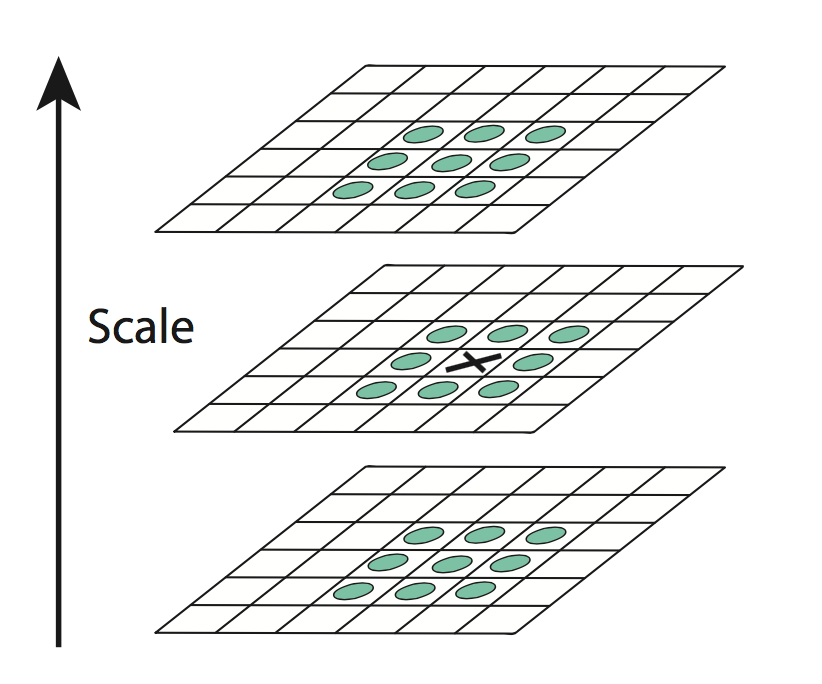
\includegraphics[width=6cm]{gfx/max}
  \caption{\cite{Lowe:2004:DIF:993451.996342} Maksima i minima wykrywane są za pomocą porównania wartości aktualnie badanego piksela (zaznaczony czarnym krzyżykiem) z jego 26 sąsiadami powstałymi poprzez złączenie kolejnych obrazów DoG z jednej oktawy. Cecha jest wykrywana w miejscu aktualnie badanego piksela jeżeli wartość tego piksela jest największa lub najmniejsza spośród 26 sąsiadów.}
  \label{fig:proponowane_algorytmy:max}
\end{figure}

\subsubsection{4. Filtrowanie cech}
\label{sec:proponowane_algorytmy:filtracja_cech}

W większości przypadków ekstrakcja cech może wygenerować ich ogromną ilość. SIFT poprzez zastosowanie następujących dwóch filtrów pozbywa się cech najgorszej jakości:

\begin{enumerate}
\item Pierwszy filtr polega na sprawdzeniu intensywności piksela obrazu DoG w miejscu gdzie wykryto cechę. Jeżeli wartość piksela jest mniejsza niż ustalony wcześniej próg cecha jest odrzucana.
\item Drugi filtr polega na obliczeniu dwóch prostopadłych do siebie gradientów w miejscu wystąpienia cechy. W zależności od otoczenia cechy możliwe są 3 opcje:
  \begin{itemize}
  \item Wartości dwóch gradientów będą małe z czego wynika, że w otoczeniu cechy jest region płaski. Cecha jest odrzucana.
  \item Wartość jednego gradientu będzie duża, a drugiego mała. Oznacza to, że wzdłuż gradientu z małą wartością występuje krawędź w oryginalnym obrazie (gradient z dużą wartością jest prostopadły do krawędzi). Cecha jest odrzucana.
  \item Wartość dwóch gradientów będzie duża. Oznacza to, że w cecha znajduje się w miejscu występowania rogu w oryginalnym obrazie. Cecha jest zachowana ze względu na to, że rogi są najlepszymi cechami.
  \end{itemize}
\end{enumerate}

\subsubsection{5. Przydzielenie orientacji cechom}
\label{sec:proponowane_algorytmy:orientacja}

Kolejny krok algorytmu SIFT polega na obliczeniu orientacji każdej cechy na podstawie jej otoczenia, przez co deskryptory cech mogą być przedstawione względnie do swojej orientacji. Dzięki temu algorytm SIFT jest niezależny od rotacji obrazów. Proces obliczenia orientacji zaczyna się od wyznaczenia wartości gradientu $m(x, y)$ i orientacji $\theta(x, y)$ dla każdego piksela z otoczenia wokół cechy za pomocą wzorów:
\begin{equation}
m(x, y) = \sqrt{(L(x + 1, y) - L(x - 1, y))^2 + (L(x, y + 1) - L(x, y - 1))^2} \\
\label{eq:magnitude}
\end{equation}
\begin{equation}
\theta(x, y) = \tan^{-1}((L(x, y + 1) - L(x, y - 1))/(L(x + 1, y) - L(x - 1, y)))
\label{eq:orientation}
\end{equation}
Następnie na podstawie wartości orientacji tworzony jest histogram posiadający 36 przedziałów przez co pokrywa zakres orientacji od 0 do 360 stopni. Każdy piksel dodany do histogramu jest ważony poprzez użycie jego wartości gradientu i wartości okrągłego okna filtra Gaussa (piksele znajdujące się dalej od cechy mają mniejszą ważność niż te znajdujące się bliżej). Orientacja odpowiadająca najwyższej wartości w histogramie jest wybrana jako orientacja cechy. Dodatkowo każda orientacja posiadająca wartość większą niż 80\% maksymalnej wartości w histogramie jest zapisywana jako nowa cecha obrazu.

\subsubsection{6. Generacja deskryptorów cech}
\label{sec:proponowane_algorytmy:deskryptor}

Deskryptor cechy musi ją charakterystycznie określać i być łatwy do obliczenia. SIFT przedstawia cechę jako 128 elementowy wektor powstały poprzez wykonanie następujących kroków:

\begin{enumerate}
\item Tworzone jest otoczenie 16 na 16 pikseli wokół cechy.
\item Dla każdego piksela w otoczeniu cechy jest liczona wartość gradientu oraz orientacja zgodnie ze wzorami \ref{eq:magnitude} i \ref{eq:orientation}. Każdą orientację piksela w otoczeniu odejmujemy od orientacji cechy obliczonej w poprzednim punkcie, przez co algorytm SIFT jest niezależny od rotacji obrazu.
\item Wartości gradientu oraz orientacji są ważone przez okrągłe okno filtru Gaussa i są następnie gromadzone poprzez utworzenie histogramu orientacji, który określa informacje w regionach 4 na 4 piksele. Rysunek \ref{fig:proponowane_algorytmy:descriptor} przedstawia proces kumulacji wartości gradientu oraz orientacji poprzez wykorzystanie histogramu.

\begin{figure}[H]
  \centering
  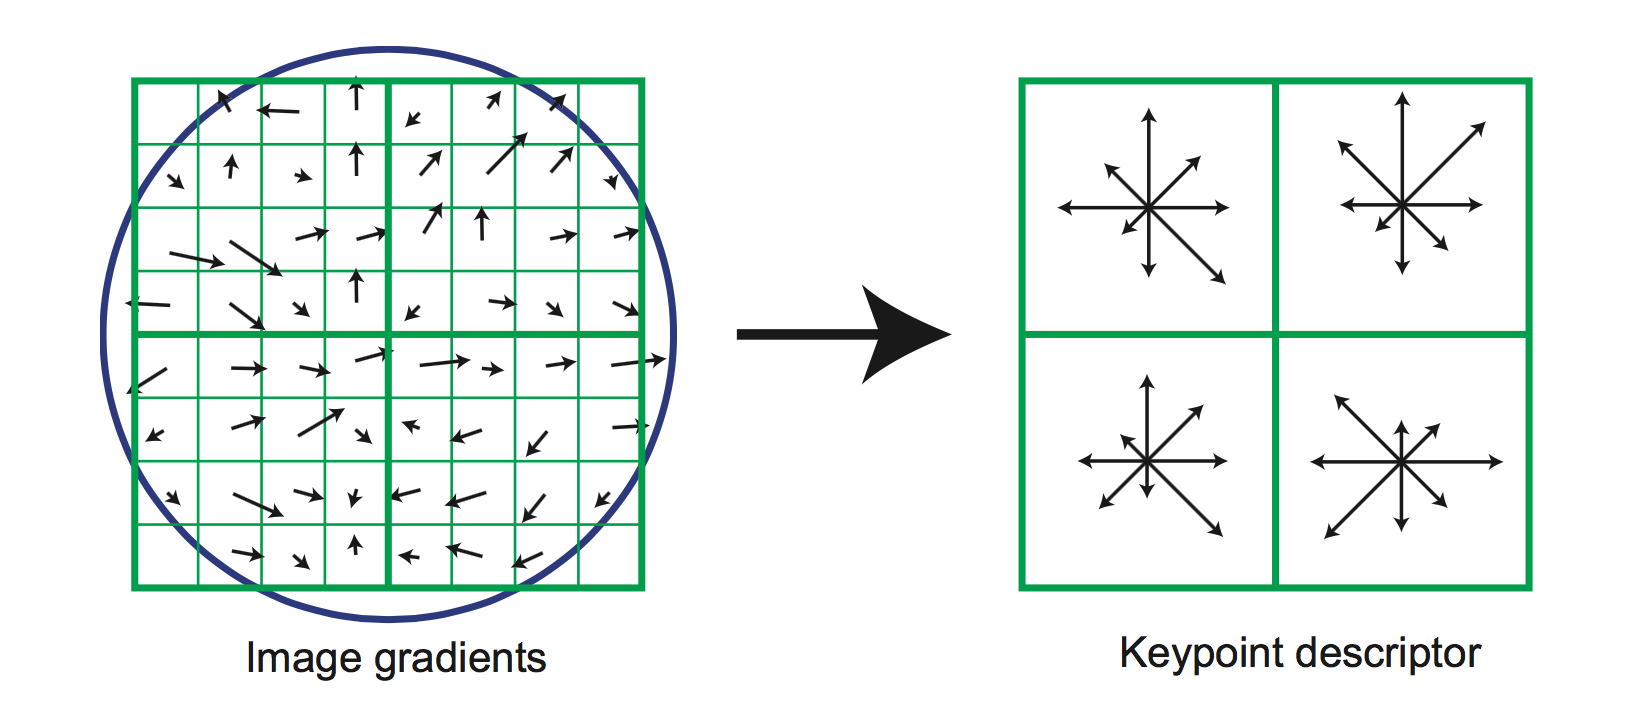
\includegraphics[width=\textwidth]{gfx/descriptor}
  \caption{\cite{Lowe:2004:DIF:993451.996342} \textbf{Lewy obraz:} Wartości orientacji oraz gradientu z uwzględnieniem okrągłego okna filtru Gaussa. \textbf{Prawy obraz:} Wartości z obszarów 4 na 4 piksele są gromadzone w histogramie, który posiada 8 przedziałów. Wartości orientacji z lewego obrazu mieszczące się w jednym przedziale histogramu są sumowane (np. piksel z orientacją 12 stopni wchodzi do przedziału 0 - 44 stopni histogramu i jego wartość jest dodawana z każdą orientacją 0 - 44 stopni).}
  \label{fig:proponowane_algorytmy:descriptor}
\end{figure}

\item Prawy obraz z rysunku \ref{fig:proponowane_algorytmy:descriptor} przedstawia deskryptor z obszaru 8 na 8 pikseli posiadający 32 elementy (4 obszary, każdy posiada 8 orientacji). Autor algorytmu SIFT podaje, że najlepsze rezultaty można uzyskać poprzez policzenie deskryptora z obszaru 16 na 16 pikseli wokół cechy, wtedy deskryptor posiada 128 elementów (16 obszarów, każdy posiada 8 orientacji).
\item Na koniec 128 elementowy wektor jest normalizowany.
\end{enumerate}

\subsubsection{Sposób wykorzystania algorytmu SIFT w programie}
\label{sec:proponowane_algorytmy:sift_wykorzystanie}

Biblioteka OpenCV posiada zaimplementowany algorytm SIFT i jego użycie sprowadza się do paru linii kodu:

\begin{verbatim}
SIFT featuresFinder = SIFT::SIFT(...);
featuresFinder(...);
\end{verbatim}

Konstruktor \texttt{SIFT::SIFT(...)} tworzy nam obiekt \texttt{SIFT} posiadający funkcjonalność algorytmu SIFT. Do konstruktora \texttt{SIFT::SIFT(...)} podajemy parametry algorytmu tj. ilość najlepszych cech do zwrócenia, ilość oktaw do wykorzystania, progi do filtrowania wykrytych cech (sekcja \ref{sec:proponowane_algorytmy:filtracja_cech}) oraz siłę filtru Gaussa. Operator \texttt{featuresFinder(...)} przyjmuje obraz w którym mają być znalezione cechy i zwraca miejsca wystąpienia tych cech oraz ich deskryptory. Więcej informacji na temat obiektu \texttt{SIFT} znajduje się w oficjalnej dokumentacji OpenCV\footnote{\url{http://docs.opencv.org/modules/nonfree/doc/feature_detection.html}}.

\subsection{Dopasowanie wyekstrahowanych cech}
\label{sec:proponowane_algorytmy:dopasowanie}

Cecha jest uważana za dopasowaną do drugiej cechy, jeżeli deskryptory (w przypadku SIFT 128 elementowy wektor) tych cech są do siebie podobne. W świecie rzeczywistym bardzo rzadko zdarza się, że deskryptory są do siebie identyczne, dlatego algorytmy zwracają zazwyczaj deskryptor, który jest najbardziej podobny. Trudność problemu dopasowania wyekstrahowanych cech jest uzależniony od ilości wykrytych cech w każdym z obrazów. Im więcej cech do dopasowania tym problem staje się bardziej kosztowny obliczeniowo. W przypadku problemu niniejszej pracy mamy do czynienia z obrazami o rozmiarze 240 na 240 pikseli z czego w większości zbiorów danych obrazy nakładają się w 10\% szerokości obrazu, czyli algorytm SIFT szuka cech w obszarze 24 na 240 pikseli. Jest to obszar na tyle mały, że ilość cech wyekstrahowanych przez SIFT jest niewielka. Dzięki temu w niniejszej pracy w procesie rejestracji kafelków każda cecha jednego obrazu jest porównywana z każdą cechą obrazu dopasowywanego. Jeżeli w jednym kafelku wykryto $n$ cech, a w drugim $m$ cech to algorytm wykonuje $nm$ dopasowań. Taki mechanizm dopasowania nazywa się \textit{Brute Force Matching} i tak jak algorytm SIFT również jest zaimplementowany w OpenCV. Użycie \textit{Brute Force Matching} w OpenCV tak jak w przypadku SIFT sprowadza się do kilku linii kodu:

\begin{verbatim}
BFMatcher bruteForceMatcher;
bruteForceMatcher.match(...);
\end{verbatim}

Obiekt \texttt{BFMatcher} posiada funkcjonalność pozwalającą na dopasowanie każdego deskryptora z jednego zbioru do każdego deskryptora z drugiego zbioru. Funkcja \texttt{match(...)} przyjmuje deskryptory z dwóch zbiorów i zwraca dopasowania. Więcej informacji na temat obiektu \texttt{BFMatcher} znajduje się w oficjalnej dokumentacji OpenCV\footnote{\url{http://docs.opencv.org/modules/features2d/doc/common_interfaces_of_descriptor_matchers.html}}.

\subsection{Filtrowanie dopasowań}
\label{sec:proponowane_algorytmy:filtrowanie}

Na tym etapie algorytm już wyekstrahował cechy z obrazów i wyznaczył dopasowania pomiędzy nimi. Ze względu na to, że naczynia krwionośne w angiograficznych obrazach OCT są bardzo do siebie podobne wiele z tych dopasowań będzie niepoprawnych. Rysunek \ref{fig:algorytmy_korejestracji:outliners} z sekcji \ref{sec:algorytmy_korejestracji:korejestracja_na_podstawie_cech} przedstawia istotę problemu niepoprawnych dopasowań, natomiast rysunek \ref{fig:proponowane_algorytmy:no_filtering} przedstawia wykryte dopasowania przez mechanizm \textit{Brute Force Matching} na dwóch rzeczywistych angiograficznych obrazach OCT.

\begin{figure}[htb]
  \centering
  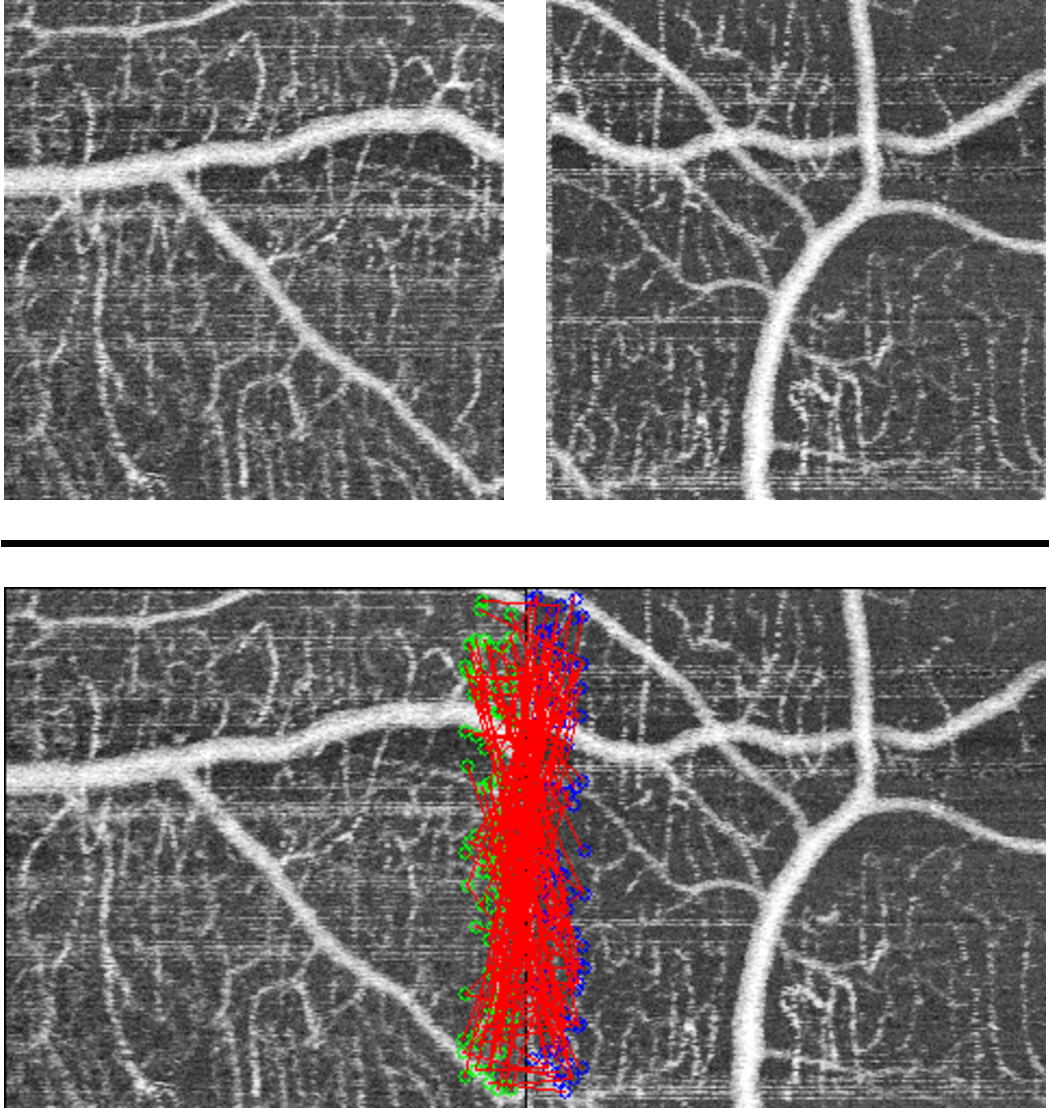
\includegraphics[width=\textwidth]{gfx/no_filtering}
  \caption{Na górze znajdują się dwa angiograficzne obrazy OCT, które mają być złączone na ok. 10\% swojej szerokości. Na dole znajdują się wykryte cechy (kółka zielone i niebieskie) w dwóch obrazach oraz znalezione dopasowania (czerwone linie) pomiędzy cechami za pomocą techniki \textit{Brute Force Matching}.}
  \label{fig:proponowane_algorytmy:no_filtering}
\end{figure}

Gołym okiem można zauważyć na podstawie rysunku \ref{fig:proponowane_algorytmy:no_filtering}, że algorytm zwrócił zdecydowanie za dużo dopasowań i znaczna ich część jest niepotrzebna. Dlatego wymagane jest dalsze filtrowanie tych dopasowań na podstawie wiedzy dziedzinowej oraz dostępnych algorytmów. Poniżej będą opisane poszczególne procesy filtrowania dopasowań w takiej kolejności w jakiej wykonuje je program.

\subsubsection{Filtrowanie na podstawie położenia}
\label{sec:proponowane_algorytmy:placement_filtering}

Pierwsza technika filtrowania polega na usunięciu dopasowań doprowadzających do przesunięcia się kafelka poza określoną normę. Ta norma jest określona poprzez dwa parametry $shiftParameter$ i $percentOverlap$, które ustawia się w pliku konfiguracyjnym. W zależności od sposobu ułożenia kafelków, dopasowanie przejdzie ten filtr jeżeli spełnia dwa warunki:

\begin{enumerate}
\item Dopasowane cechy nie będą się znajdować zbyt daleko od siebie w osi poziomej (w przypadku ułożenia kafelków w pionie) lub osi pionowej (w przypadku ułożenia kafelków w poziomie). Ten warunek określają wzory -- \ref{eq:vertical} dla przypadku ułożenia kafelków w pionie, \ref{eq:horizontal} dla przypadku ułożenia kafelków w poziomie:
\begin{equation}
\left|f_{1x} - f_{2x}\right| < imageSize * shiftParameter
\label{eq:vertical}
\end{equation}
\begin{equation}
\left|f_{1y} - f_{2y}\right| < imageSize * shiftParameter
\label{eq:horizontal}
\end{equation}
Gdzie $f_{1x}$ i $f_{2x}$ to współrzędne $x$ dopasowanych cech z dwóch obrazów (dla $f_{1y}$ i $f_{2y}$ są to współrzędne $y$), a $imageSize$ to rozmiar angiograficznego obrazu OCT (w przypadku niniejszej pracy ma 240 pikseli).
\item Dopasowane cechy nie będą znajdować się zbyt daleko od siebie. Ten warunek określa wzór:
\begin{equation}
length < imageSize * percentOverlap * 2.5
\label{eq:length}
\end{equation}
Gdzie $length$ to długość wektora pomiędzy cechami z uwzględnieniem położenia kafelków. W zależności od położenia kafelków $length$ jest zdefiniowane jako -- \ref{eq:left} dla położenia, w którym kafelki ustawione są w poziomie i kafelek $f_{1}$ znajduje się z lewej strony kafelka $f_{2}$, \ref{eq:up} dla położenia, w którym kafelki ustawione są w pionie i kafelek $f_{1}$ znajduje się nad kafelkiem $f_{2}$:
\begin{equation}
length = \sqrt{(f_{1x} - (f_{2x} + imageSize))^2 + (f_{1y} - f_{2y})^2}
\label{eq:left}
\end{equation}
\begin{equation}
length = \sqrt{(f_{1x} - f_{2x})^2 + (f_{1y} - (f_{2y} + imageSize))^2}
\label{eq:up}
\end{equation}
\end{enumerate}

Rysunek \ref{fig:proponowane_algorytmy:after_placement} przedstawia wynik filtracji na tych samych dwóch obrazach angiograficznych użytych jako przykład w rysunku \ref{fig:proponowane_algorytmy:no_filtering}.

\begin{figure}[htb]
  \centering
  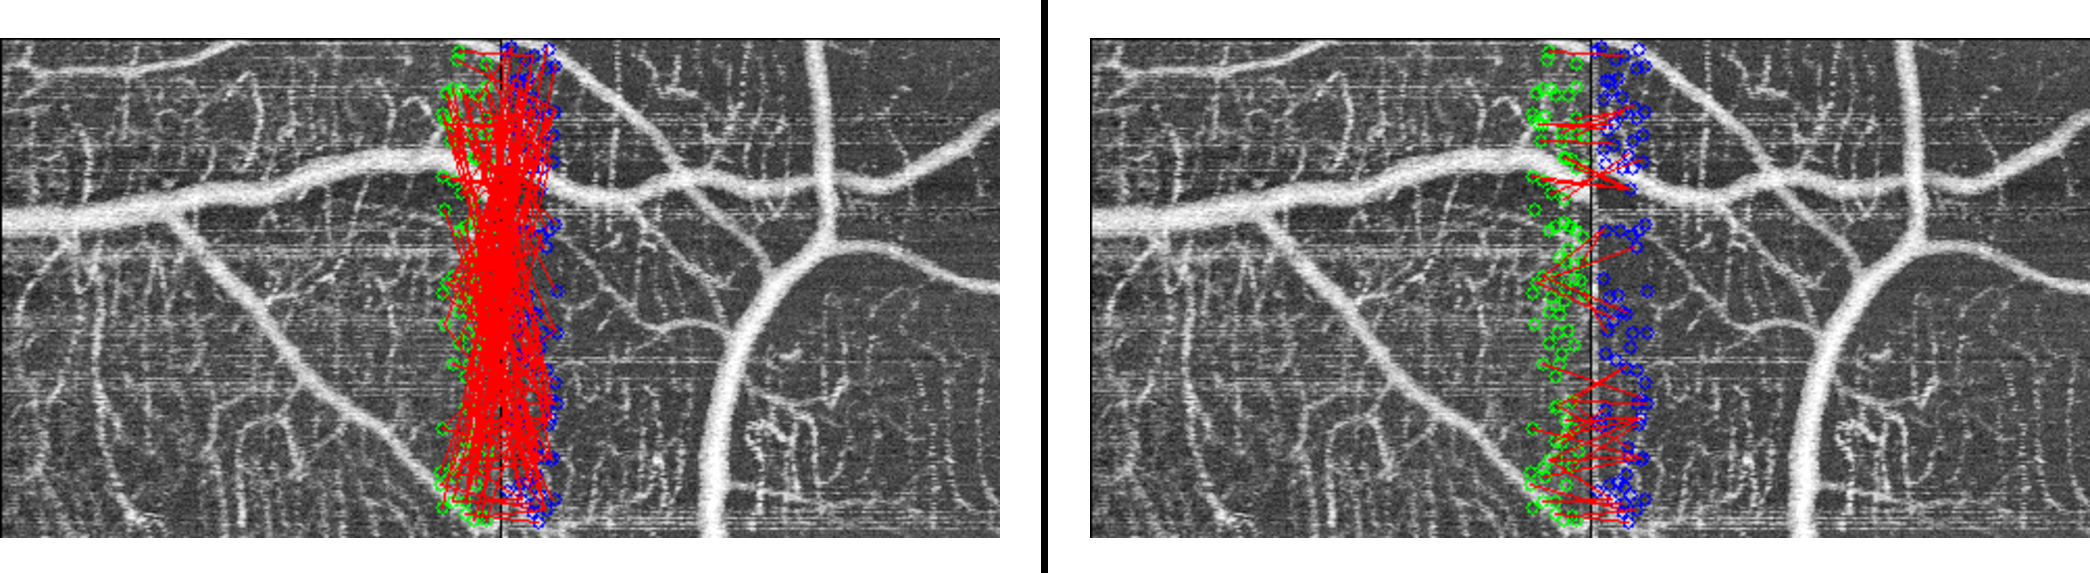
\includegraphics[width=\textwidth]{gfx/after_placement}
  \caption{\textbf{Górny obraz:} Dopasowania wyznaczone po zastosowaniu \textit{Brute Force Matching}. \textbf{Dolny obraz:} Dopasowania pozostałe po filtrowaniu na podstawie położenia.}
  \label{fig:proponowane_algorytmy:after_placement}
\end{figure}

\subsubsection{Usuwanie nadmiarowych dopasowań przypisanych do jednej cechy}
\label{sec:proponowane_algorytmy:no_repetition_filtering}

Czasem występuje sytuacja, w której jedną cechę z jednego kafelka dopasowano do kilku cech z drugiego kafelka. Na podstawie wiedzy dziedzinowej wiemy, że jest to sytuacja niepożądana i cecha może być dopasowana tylko i wyłącznie do jednej cechy. Niniejszy etap filtracji polega na iteracji po wszystkich cechach posiadających dopasowania do więcej niż jednej cechy i na pozostawieniu tylko najbardziej podobnej cechy (na podstawie wartości deskryptoru cechy). Ten etap filtrowania jest wykonywany dwukrotnie -- pierwszy raz dla cech z pierwszego kafelka i drugi raz dla cech z drugiego kafelka. Rysunek \ref{fig:proponowane_algorytmy:no_repetition_filtering} przedstawia wynik filtracji poprzez eliminację nadmiarowych dopasowań na dopasowaniach będących wynikiem filtracji poprzedniej (rysunek \ref{fig:proponowane_algorytmy:after_placement}).

\begin{figure}[htb]
  \centering
  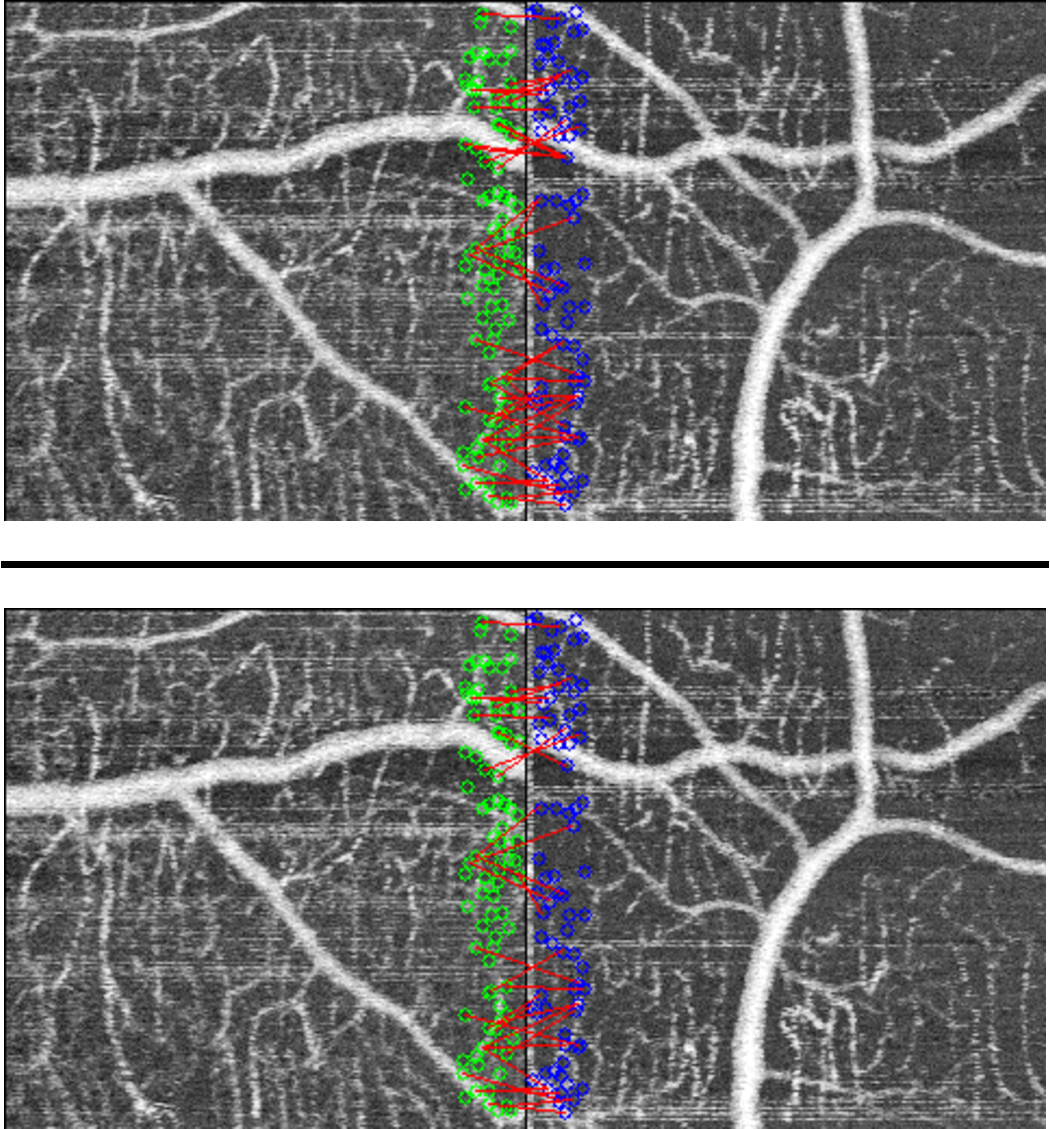
\includegraphics[width=\textwidth]{gfx/no_repetition_filtering}
  \caption{\textbf{Górny obraz:} Dopasowania wyznaczone po zastosowaniu filtrowania na podstawie położenia. \textbf{Dolny obraz:} Dopasowania pozostałe po eliminacji nadmiarowych dopasowań.}
  \label{fig:proponowane_algorytmy:no_repetition_filtering}
\end{figure}

\subsubsection{RANSAC}
\label{sec:proponowane_algorytmy:ransac}

Poprzednie dwa kroki filtrowania dopasowań wyeliminowały znaczącą część dopasowań wykrytych na początku. Niestety nadal można zauważyć (prawy obraz na rysunku \ref{fig:proponowane_algorytmy:no_repetition_filtering}), że niektóre dopasowania są nieprawidłowe. Algorytm RANSAC (ang. \textit{random sample consensus, RANSAC}) pierwszy raz opublikowany w roku 1981 przez Fischler i Bolles \cite{Fischler:1981:RSC:358669.358692} zaimplementowano by wyeliminować próbki tworzące szum w znalezieniu poprawnego modelu. W niniejszej pracy próbkami są dopasowania cech, a modelem jest poprawna macierz transformacji pomiędzy kafelkami.

Działanie algorytmu RANSAC składa się z dwóch kroków powtarzanych w sposób iteracyjny:

\begin{enumerate}
\item W pierwszym kroku algorytm losowo wybiera podzbiór próbek. Następnie używając tylko próbek z tego podzbioru oblicza pasujący model.
\item W drugim kroku algorytm sprawdza, które próbki z całego zbioru są zgodne z modelem obliczonym w pierwszym kroku. Próbka będzie uznana za szum jeżeli nie będzie pasować do modelu w obrębie progu błędu.
\end{enumerate}

Algorytm RANSAC będzie powtarzał powyższe dwa kroki dopóki nie znajdzie w kroku drugim wystarczającej ilości próbek pasujących do modelu wyznaczonego w kroku pierwszym lub nie przekroczy liczby iteracji, która jest parametrem algorytmu. Rysunek \ref{fig:proponowane_algorytmy:ransac} \footnote{\url{https://en.wikipedia.org/wiki/RANSAC}} przedstawia działanie algorytmu RANSAC na problemie, w którym próbkami są punkty, a szukanym modelem jest funkcja prostej.

\begin{figure}[htb]
  \centering
  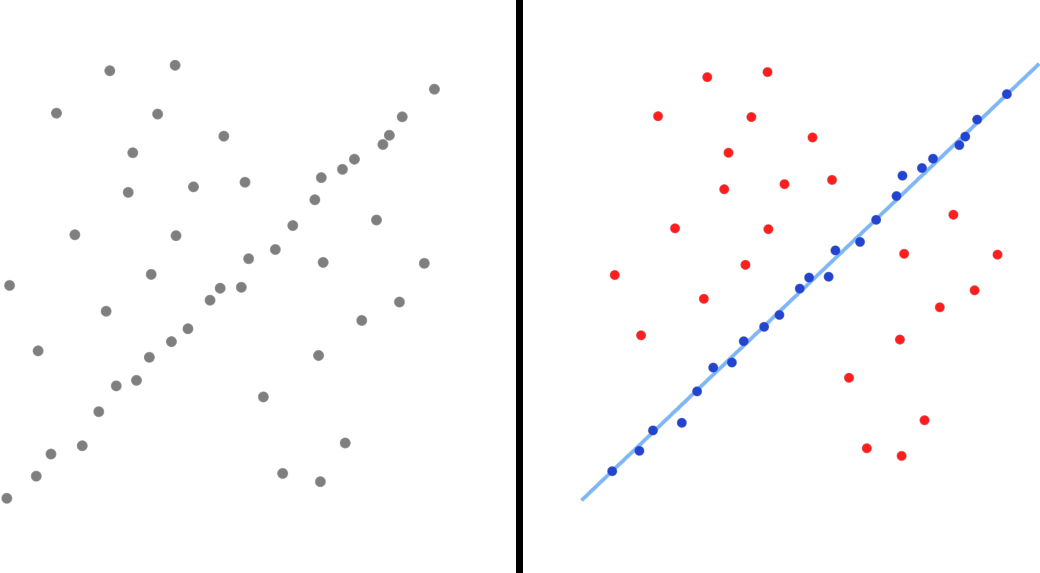
\includegraphics[width=8cm]{gfx/ransac}
  \caption{\textbf{Lewy obraz:} Zbiór danych, w którym wiele punktów jest szumem. \textbf{Prawy obraz:} Funkcja prostej (niebieska linia) obliczona przez algorytm RANSAC. Punkty, które są szumem (czerwone kropki) nie mają wpływu na model, czyli funkcję prostej.}
  \label{fig:proponowane_algorytmy:ransac}
\end{figure}

Biblioteka OpenCV implementuje algorytm RANSAC w sposób niejawny wewnątrz funkcji \texttt{findHomography(...)}, której celem jest znalezienie afinicznej transformacji pomiędzy dwoma zbiorami punktów. Dodatkowo funkcja \texttt{findHomography(...)} implementuje krok pozbywający się szumu ze swoich danych wejściowych. Ten krok może być wykonany za pomocą metody RANSAC lub LMedS (ang. \textit{least-median of squares, LMedS}). Żeby otrzymać wynik algorytmu RANSAC na dopasowaniach pomiędzy punktami \texttt{featuresSource} z pierwszego kafelka i \texttt{featuresTarget} z drugiego kafelka należy do funkcji \texttt{findHomography(...)} przekazać opcjonalny wektor \texttt{mask}, w którym będzie zapisany wynik algorytmu RANSAC. Wywołanie funkcji wygląda następująco:

\begin{verbatim}
findHomography(featuresSource, featuresTarget, CV_RANSAC, 3, mask)
\end{verbatim}

Wartość \texttt{CV\_RANSAC} powoduje użycie algorytmu RANSAC zamiast LMedS. Jeżeli element o indeksie $i$ wektora \texttt{mask} posiada wartość, która jest równa $0$ to cechy o indeksie $i$ wektorów \texttt{featuresSource} i \texttt{featuresTarget} są szumem.

Rysunek \ref{fig:proponowane_algorytmy:ransac_filter} przedstawia wynik algorytmu RANSAC na dopasowaniach będących wynikiem poprzedniego procesu filtracji (rysunek \ref{fig:proponowane_algorytmy:no_repetition_filtering}).

\begin{figure}[htb]
  \centering
  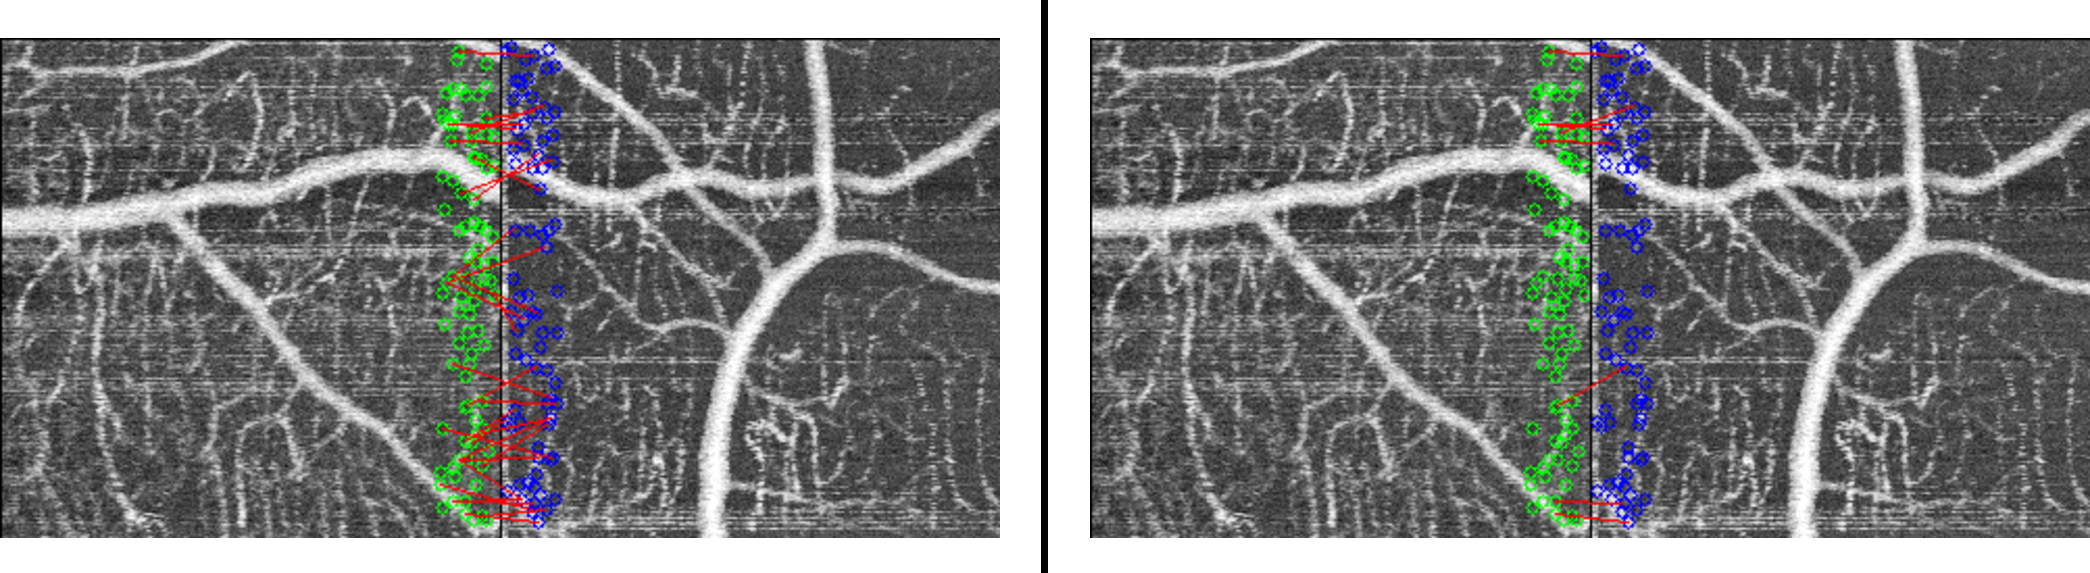
\includegraphics[width=\textwidth]{gfx/ransac_filter}
  \caption{\textbf{Górny obraz:} Dopasowania pozostałe po eliminacji nadmiarowych dopasowań. \textbf{Dolny obraz:} Dopasowania pozostałe po użyciu algorytmu RANSAC.}
  \label{fig:proponowane_algorytmy:ransac_filter}
\end{figure}

\subsubsection{Filtrowanie na podstawie nachylenia linii dopasowania}
\label{sec:proponowane_algorytmy:slope_filtering}

Ostatni etap filtrowania składa się z trzech kroków:

\begin{enumerate}
\item Dla każdego dopasowania obliczany jest kąt nachylenia $angle$ funkcji prostej przechodzącej przez cechy z tego dopasowania. W zależności od ułożenia kafelków cechy mają współrzędne odpowiednio zmodyfikowane poprzez rozmiar kafelka.
\item Z obliczonych w poprzednim kroku wartości kątów nachylenia wyznaczana jest wartość mediany $medianAngle$.
\item Dopasowanie przechodzi ten filtr jeżeli kąt nachylenia $angle$ obliczony w pierwszym kroku zawiera się w przedziale ograniczonym przez wartość mediany $medianAngle$ wyznaczonej w kroku drugim i parametr $angleParameter$, który ustawia się w pliku konfiguracyjnym:
\begin{equation}
medianAngle + angleParameter > angle > medianAngle - angleParameter
\label{eq:angle}
\end{equation}
\end{enumerate}

Filtr ma na celu pozostawić dopasowania z podobnym nachyleniem. Rysunek \ref{fig:proponowane_algorytmy:slope} przedstawia wynik filtrowania na podstawie nachylenia dopasowań będących wynikiem poprzedniego procesu filtracji (rysunek \ref{fig:proponowane_algorytmy:ransac_filter}).

\begin{figure}[H]
  \centering
  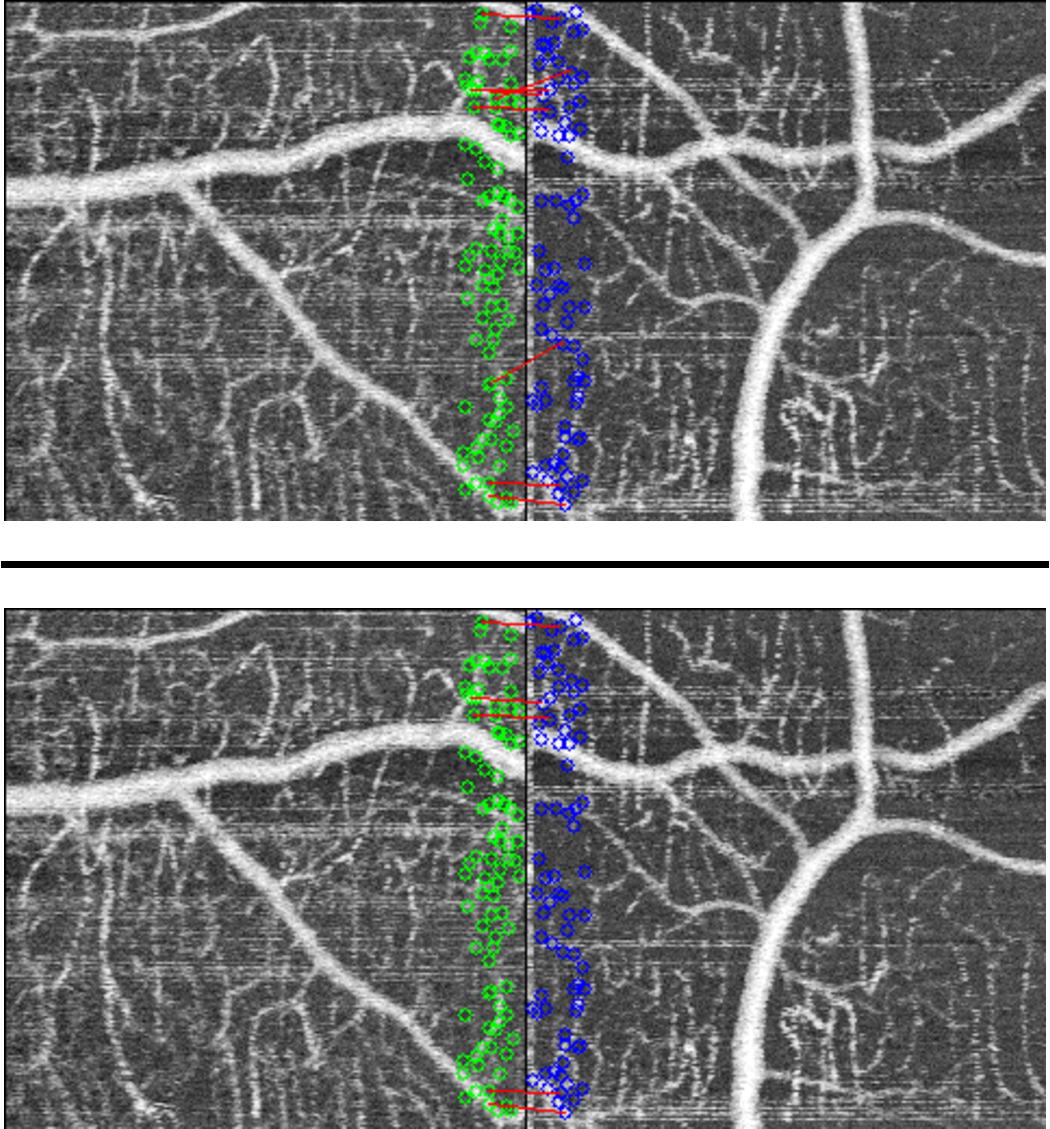
\includegraphics[width=\textwidth]{gfx/slope}
  \caption{\textbf{Górny obraz:} Dopasowania pozostałe po użyciu algorytmu RANSAC. \textbf{Dolny obraz:} Dopasowania posiadające podobny kąt nachylenia.}
  \label{fig:proponowane_algorytmy:slope}
\end{figure}

Wynik ostatniego filtru przedstawiony na prawym obrazie na rysunku \ref{fig:proponowane_algorytmy:slope} pozostawia poprawne dopasowania, które mogą być użyte do estymacji macierzy transformacji (sekcja \ref{sec:proponowane_algorytmy:estymacja}).

\section{Rejestracja kafelków poprzez wykrycie położeń naczyń krwionośnych w kafelkach}
\label{sec:proponowane_algorytmy:depth_first_search}

Technika rejestracji kafelków za pomocą cech opisana w sekcji \ref{sec:proponowane_algorytmy:cechy} jest jedną z dwóch metod rejestracji zaimplementowanych w programie. Niniejszy rozdział przedstawia drugą metodę, która została zaimplementowana ze względu na pojawienie się zbioru kafelków o niestandardowym rozmiarze tj. 40 na 240 pikseli. Dla takiego zbioru szerokość obszaru nałożenia wynosi 4 piksele co jest zdecydowanie zbyt małą wartością by wykryć cechy. By zarejestrować kafelki w takim rozmiarze należało wziąć pod uwagę obszar całego kafelka, a nie tylko obszar nałożenia. Metoda zaproponowana w niniejszej sekcji ma na celu wykrycie miejsc występowania naczyń krwionośnych na krawędziach obrazu kafelka. Wynik tej metody jest przedstawiony na rysunku \ref{fig:proponowane_algorytmy:paths_detected}.

\begin{figure}[H]
  \centering
  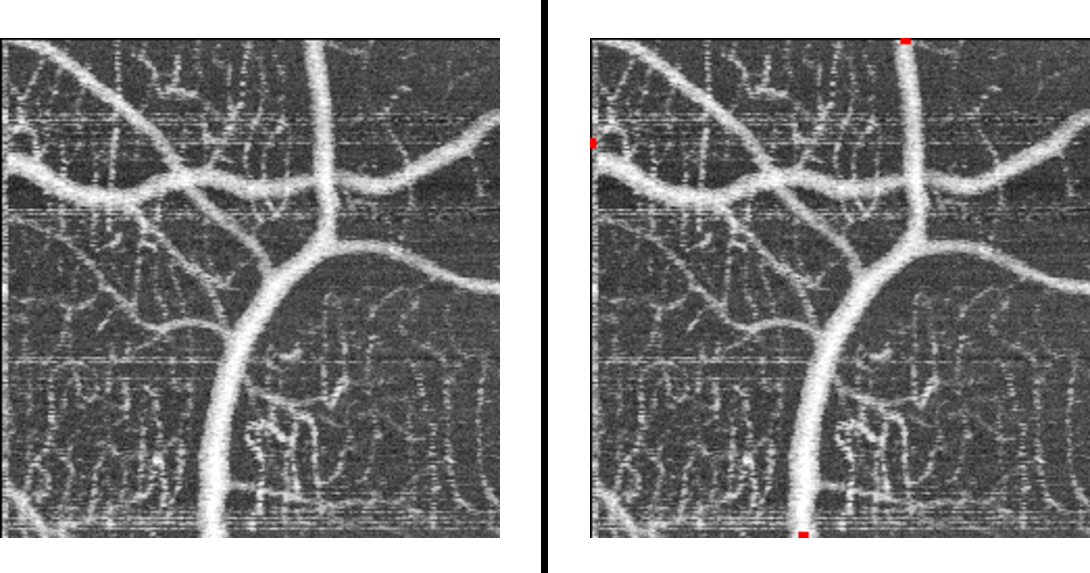
\includegraphics[width=8cm]{gfx/paths_detected}
  \caption{\textbf{Lewy obraz:} Przykładowy angiograficzny obraz OCT. \textbf{Prawy obraz:} Wykryte naczynia krwionośne na krawędziach obrazu (zaznaczone czerwonymi prostokątami).}
  \label{fig:proponowane_algorytmy:paths_detected}
\end{figure}

W sekcji \ref{sec:proponowane_algorytmy:zasada_dzialania} opisano zasadę działania algorytmu.

\subsection{Zasada działania}
\label{sec:proponowane_algorytmy:zasada_dzialania}

Działanie algorytmu można podzielić na dwa etapy:

\subsubsection{1. Tworzenie szkieletu obrazu angiograficznego}

Szkieletem obiektu nazywamy kształt znajdujący się wewnątrz tego obiektu, którego krawędzie są równo oddalone od krawędzi obiektu. Przykład szkieletu znajduje się na rysunku \ref{fig:proponowane_algorytmy:skel}\footnote{\url{https://en.wikipedia.org/wiki/Topological_skeleton}}.

\begin{figure}[H]
  \centering
  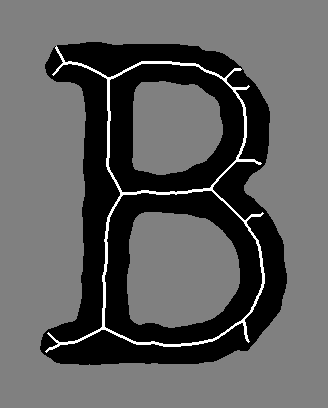
\includegraphics[width=2cm]{gfx/skel}
  \caption{Szkielet (zaznaczony białą linią) litery B.}
  \label{fig:proponowane_algorytmy:skel}
\end{figure}

Szkielet naczynia krwionośnego idealnie oddaje jego pozycje poprzez wyznaczenie jego środka. Proces tworzenia szkieletu obrazu angiograficznego zaczyna się od wstępnego przetwarzania (rysunek \ref{fig:proponowane_algorytmy:preprocess}) składającego się z dwóch etapów:

\begin{enumerate}
\item Binaryzacji obrazu.
\item Zastosowania operacji morfologicznych na obrazie (zamknięcie, a następnie otwarcie).
\end{enumerate}

\begin{figure}[H]
  \centering
  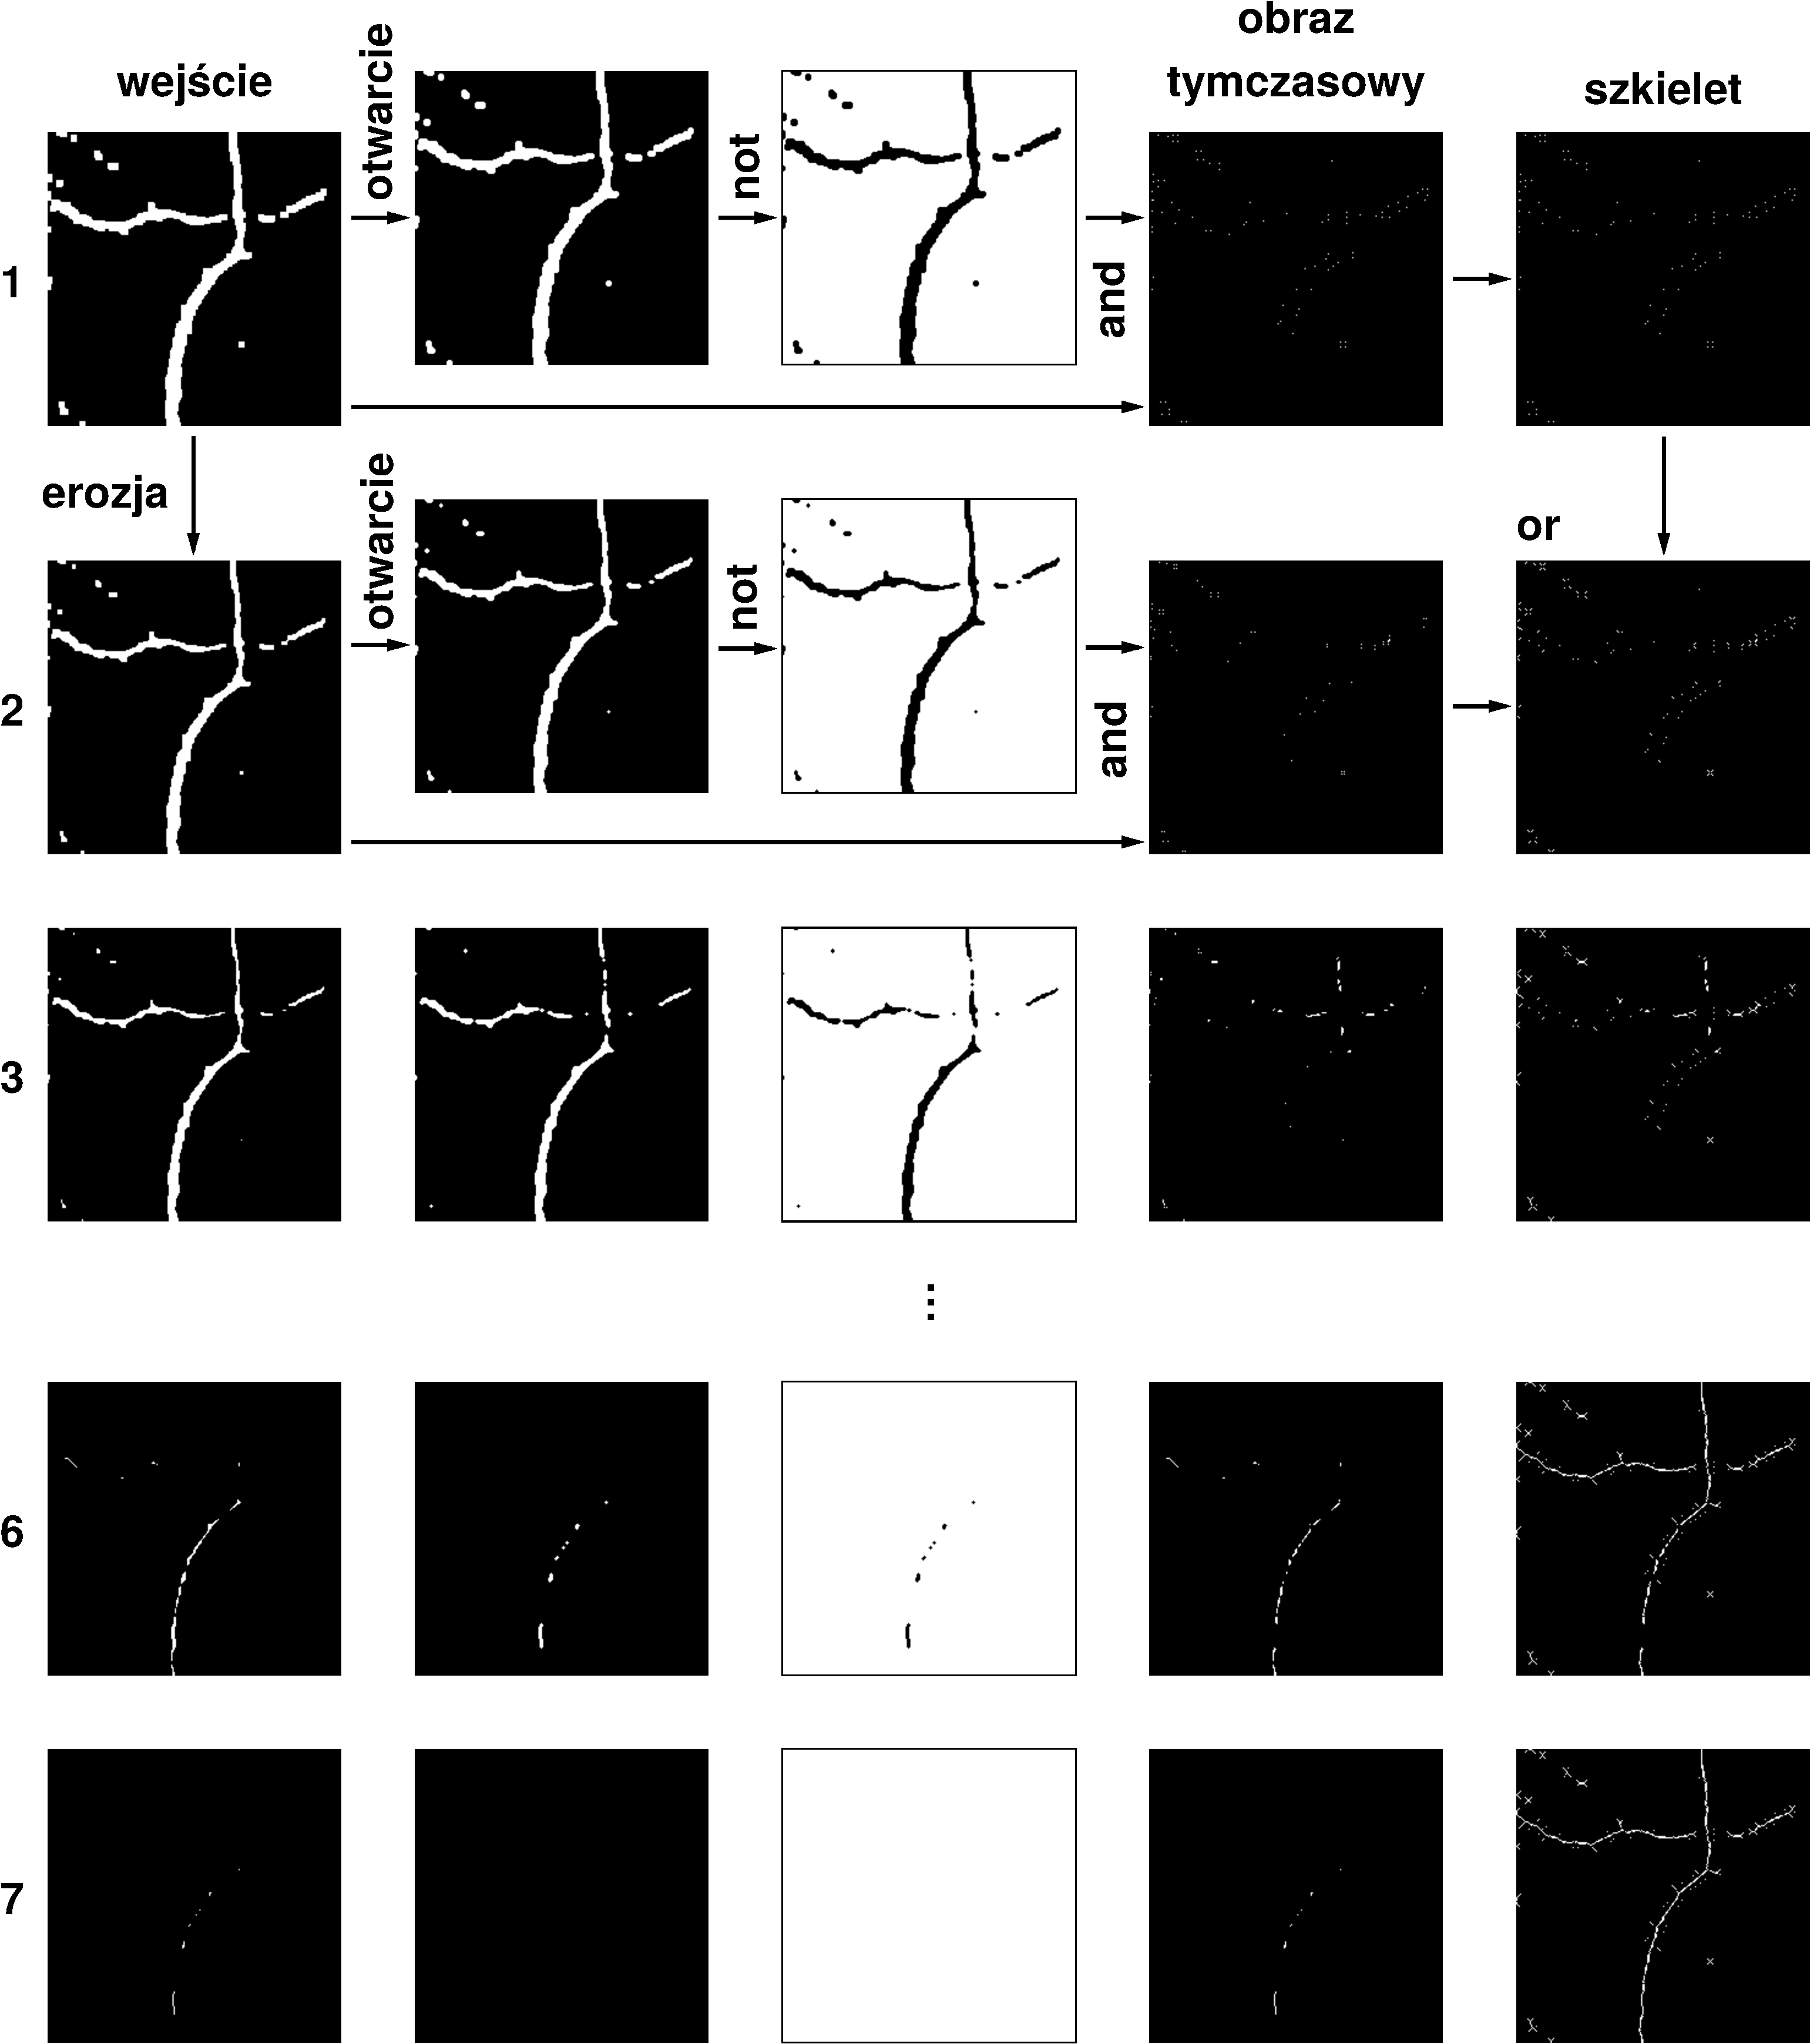
\includegraphics[width=\textwidth]{gfx/skeleton}
  \caption{Rysunek przedstawia przykładowy proces tworzenia szkieletu. Obraz w lewym górnym rogu jest obrazem wejściowym i jest wynikiem wstępnego przetwarzania. Algorytm potrzebował w tym przypadku 7 iteracji by stworzyć szkielet (iteracje są zaznaczone numerami z lewej strony). W każdej iteracji proces zaczyna się od otwarcia, a następnie negacji obrazu wejściowego (obraz w 1 kolumnie). Wynik poprzedniej operacji wraz z obrazem wejściowym jest poddany operatorowi logicznemu \textit{and}, którego wynik jest zapisany w obrazie tymczasowym (obraz w 4 kolumnie). Szkielet powstaje poprzez zastosowanie operatora logicznego \textit{or} na szkielecie z poprzedniej iteracji i obrazie tymczasowym z aktualnej iteracji. Po każdej iteracji obraz wejściowy jest poddawany erozji. Algorytm kończy działanie, jeżeli obraz wejściowy po operacji erozji będzie posiadał wszystkie piksele o wartości 0. Obraz w prawym dolnym rogu jest wynikiem algorytmu oraz finalnym szkieletem.}
  \label{fig:proponowane_algorytmy:skeleton}
\end{figure}

\begin{figure}[H]
  \centering
  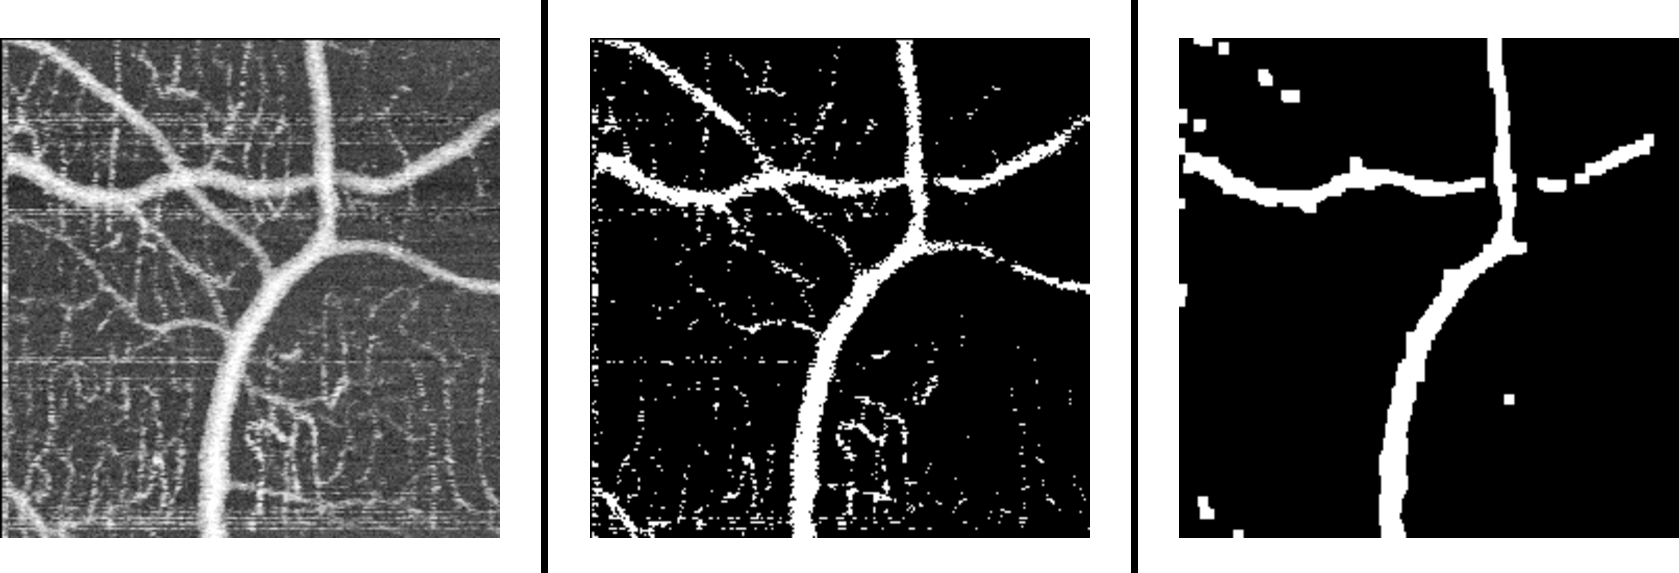
\includegraphics[width=9cm]{gfx/preprocess}
  \caption{\textbf{Lewy obraz:} Przykładowy angiograficzny obraz OCT. \textbf{Środkowy obraz:} Wynik binaryzacji obrazu z progiem o wartości 180. \textbf{Prawy obraz:} Wynik operacji morfologicznych z elementem strukturalnym 3 na 3 piksele dla zamknięcia i 5 na 5 pikseli dla otwarcia.}
  \label{fig:proponowane_algorytmy:preprocess}
\end{figure}

Kolejnym krokiem jest proces stworzenia szkieletu na obrazie wynikowym powstałym po wstępnym przetwarzaniu. Proces składa się z 6 etapów, które wykonywane są pętli do momentu stworzenia szkieletu. Technika jest zobrazowana oraz wyjaśniona na rysunku \ref{fig:proponowane_algorytmy:skeleton}.

\subsubsection{2. Eksploracja szkieletu za pomocą \textit{depth first search}}

Szkielet obrazu angiograficznego OCT jest następnie wykorzystany do wykrycia położeń naczyń krwionośnych. Proces rozpoczyna się od ustalenia położeń białych pikseli na krawędziach szkieletu (są to potencjalne miejsca, w których może zacząć się naczynie krwionośne). Następnie algorytm rozpoczyna eksploracje podążając białymi pikselami szkieletu z wykorzystaniem techniki \textit{depth first serach}\footnote{\url{https://en.wikipedia.org/wiki/Depth-first_search}}, dzięki czemu eksploracja wzdłuż naczynia krwionośnego przebiega szybciej. Algorytm wykrywa naczynie krwionośne jeżeli dojdzie do piksela $p$ spełniającego warunki w zależności od początku drogi eksploracji -- \ref{eq:up_or_down} dla początku w górnej lub dolnej krawędzi obrazu, \ref{eq:left_or_right} dla początku w lewej lub prawej krawędzi obrazu.
\begin{equation}
distance > imageSize * 0.5 \wedge \left|p_{y} - startp_{y}\right| > 0.1 * imageSize
\label{eq:up_or_down}
\end{equation}
\begin{equation}
distance > imageSize * 0.5 \wedge \left|p_{x} - startp_{x}\right| > 0.1 * imageSize
\label{eq:left_or_right}
\end{equation}
Gdzie $imageSize$ to rozmiar obrazu (w przypadku niniejszej pracy jest to 240 pikseli), $startp$ to piksel od którego rozpoczęła się eksploracja, a $distance$ to odległość euklidesowa pomiędzy $p$, a $startp$. Współrzędne $p.x$, $p.y$, $startp_{x}$ i $startp_{y}$ są wyrażone w układzie współrzędnych z początkiem w lewym górnym rogu obrazu.

Rysunek \ref{fig:proponowane_algorytmy:path_explor} przedstawia przykładową eksplorację szkieletu.

\begin{figure}[htb]
  \centering
  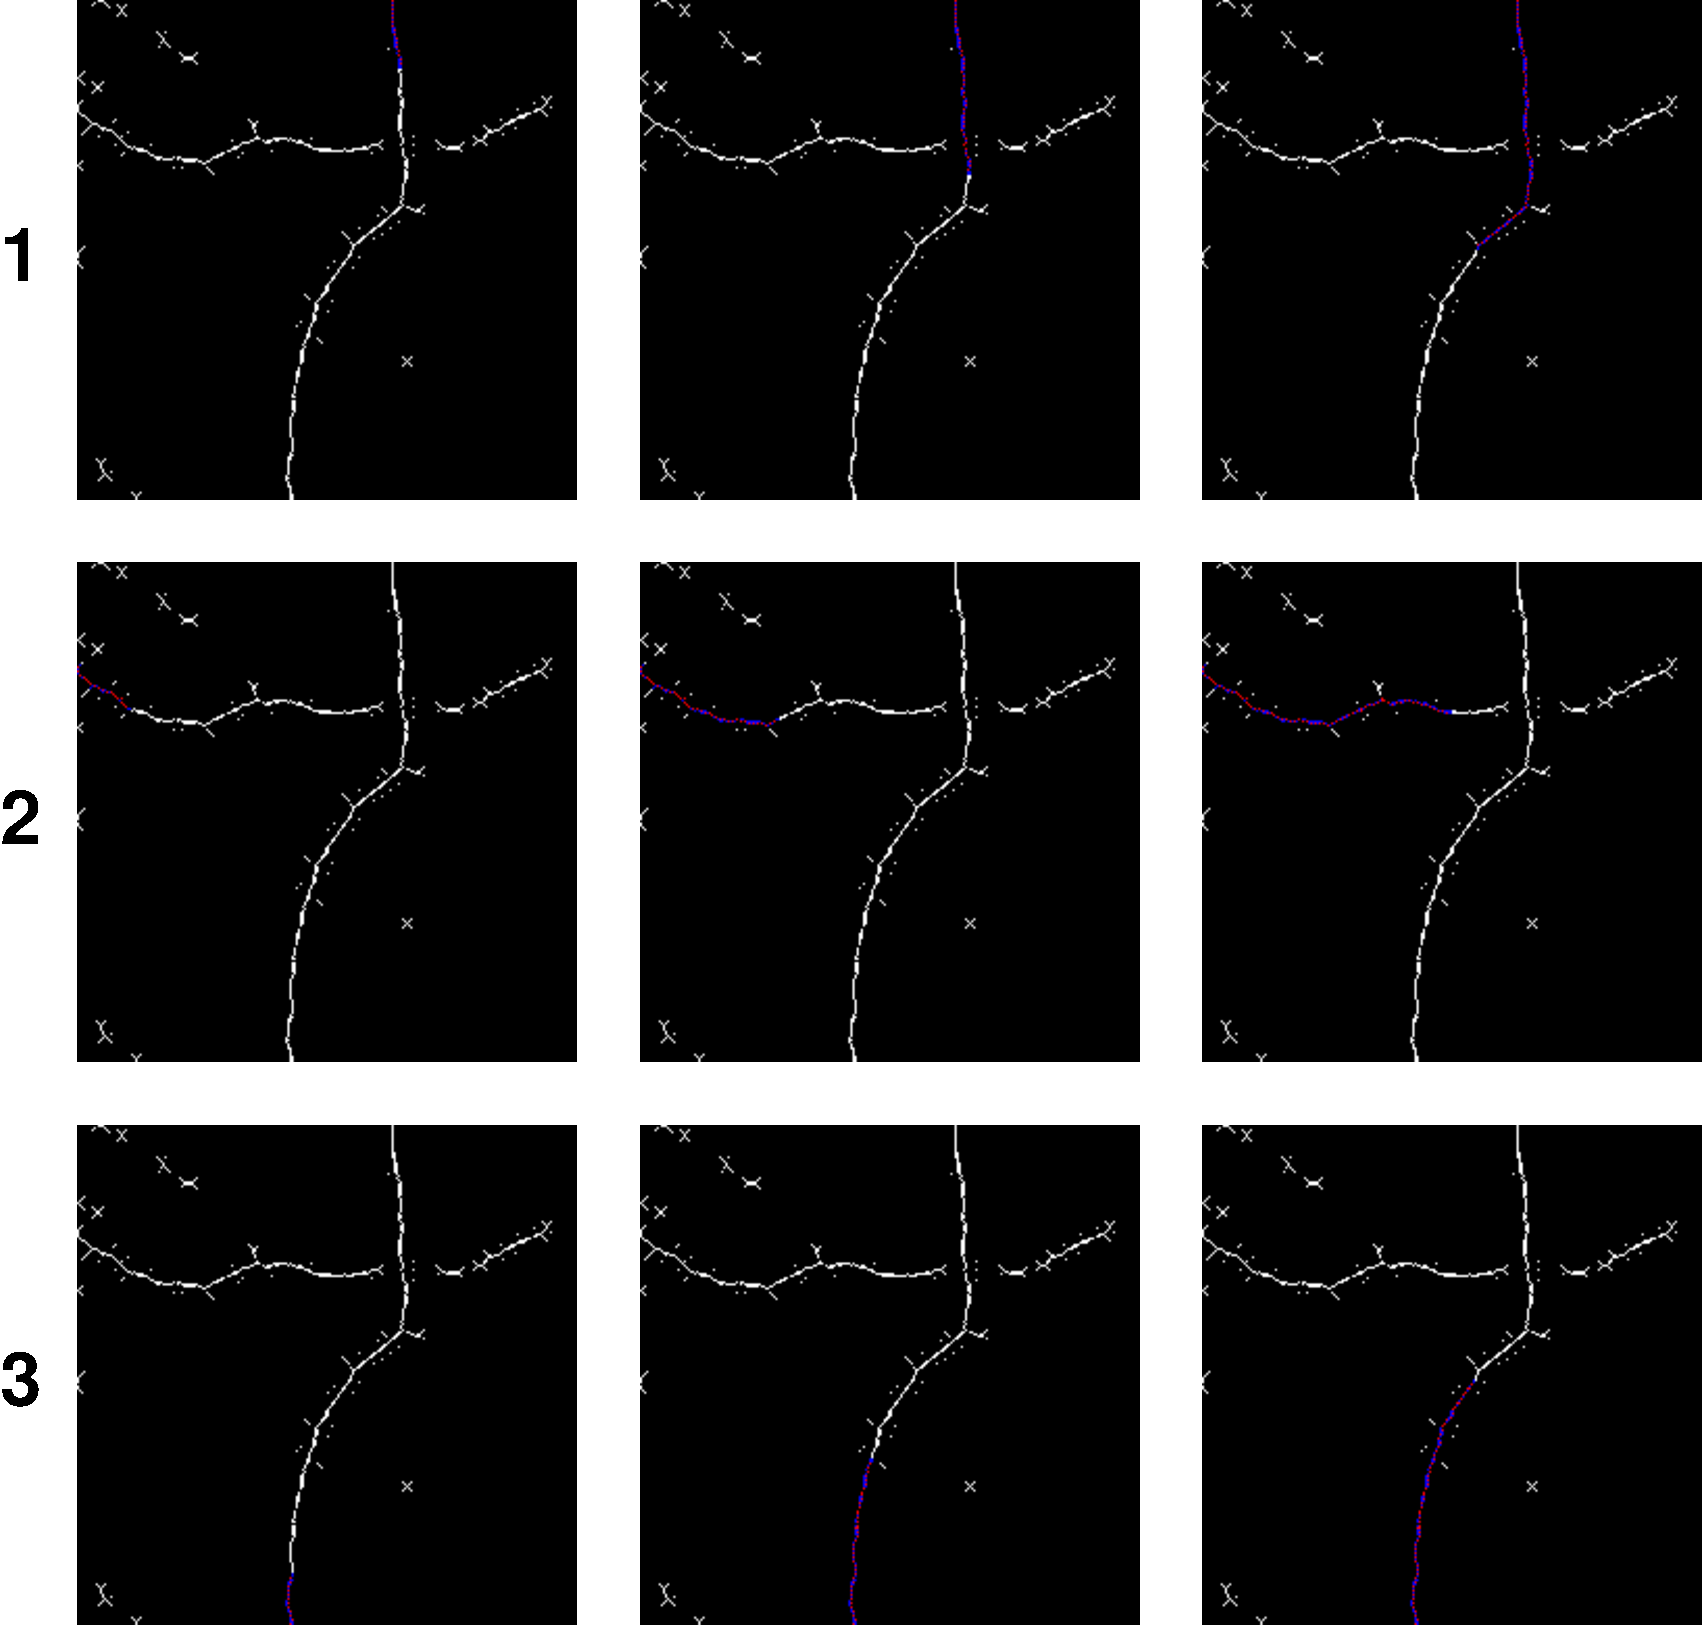
\includegraphics[width=9cm]{gfx/path_explor}
  \caption{Odkrywanie naczyń krwionośnych w różnych momentach działania algorytmu w zależności od początku eksploracji. Każdy rząd reprezentuje inne naczynie krwionośne. Wynik eksploracji jest przedstawiony w prawym obrazie na rysunku \ref{fig:proponowane_algorytmy:paths_detected}.}
  \label{fig:proponowane_algorytmy:path_explor}
\end{figure}

\section{Estymacja macierzy transformacji pomiędzy kafelkami}
\label{sec:proponowane_algorytmy:estymacja}

W programie zaimplementowano cztery metody wyznaczające macierz transformacji pomiędzy dwoma kafelkami. W niniejszej sekcji opisano każdą z nich. Proces decyzyjny opisany w sekcji \ref{sec:proponowane_algorytmy:proces_decyzyjny} określa która z czterech metod zostanie wykorzystana przez program.

\subsection{Estymacja macierzy transformacji na podstawie wykrytych naczyń krwionośnych}
\label{sec:proponowane_algorytmy:use_paths}

Metoda wykrywająca naczynia krwionośne opisana w sekcji \ref{sec:proponowane_algorytmy:depth_first_search} została zaimplementowana ze względu na pojawienie się niestandardowego zbioru danych z kafelkami o rozmiarze 40 na 240 pikseli. Wyjściem metody jest zbiór punktów wskazujący miejsce występowania naczynia krwionośnego na krawędzi obrazu, które przez resztę tej sekcji są nazywane punktami charakterystycznymi. Przykładowo punkt o współrzędnych $(24, 0)$ informuje algorytm, że naczynie krwionośne zaczyna się lub kończy w tym punkcie.

Proces estymacji macierzy transformacji jest zależny od relacji pomiędzy dwoma kafelkami. Rysunek \ref{fig:proponowane_algorytmy:path_trans} przedstawia przykładową relację kafelek z zaznaczonymi wykrytymi naczyniami krwionośnymi oraz wynik transformacji wyznaczoną macierzą.

\begin{figure}[H]
  \centering
  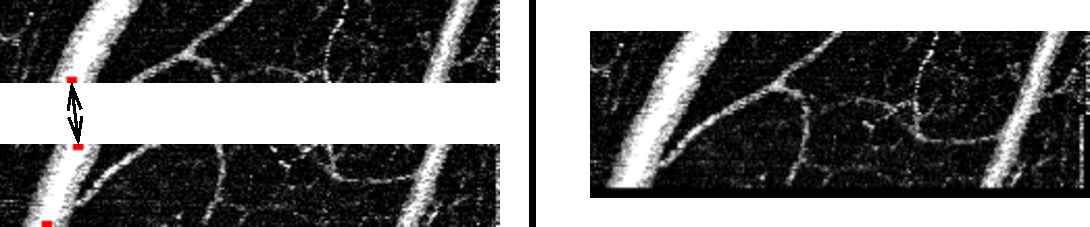
\includegraphics[width=9cm]{gfx/path_trans}
  \caption{\textbf{Lewy obraz:} Przykładowe dwa obrazy z zaznaczonymi wykrytymi naczyniami krwionośnymi. Czarna strzałka wskazuje punkty charakterystyczne użyte do wyznaczenia macierzy transformacji. \textbf{Prawy obraz:} Wynik zaaplikowania wyznaczonej macierzy transformacji (z dodatkowym łączeniem opisanym w sekcji \ref{sec:proponowane_algorytmy:laczenie_kafelkow}.}
  \label{fig:proponowane_algorytmy:path_trans}
\end{figure}

By wyznaczyć macierz transformacji algorytm wybiera punkty charakterystyczne leżące najbliżej lewej krawędzi (dla relacji kafelków z rysunku \ref{fig:proponowane_algorytmy:path_trans}) lub leżące najbliżej górnej krawędzi (dla kafelków ustawionych poziomo). Wybrane punkty charakterystyczne $p_{1}$ i $p_{2}$ należą do tego samego naczynia krwionośnego jeżeli różnica ich odpowiednich współrzędnych mieści się w ustalonym przedziale $range$ -- \ref{eq:path_up_or_down} dla ułożenia pionowego, \ref{eq:path_left_or_right} dla ułożenia poziomego.
\begin{equation}
\left|p_{1x}- p_{2x}\right| < range
\label{eq:path_up_or_down}
\end{equation}
\begin{equation}
\left|p_{1y} - p_{2y}\right| < range
\label{eq:path_left_or_right}
\end{equation}
Na podstawie zweryfikowanych punktów charakterystycznych macierz transformacji $T$ wyznacza się następująco -- \ref{eq:trans_matrix_up_or_down} dla ułożenia pionowego, \ref{eq:trans_matrix_left_or_right} dla ułożenia poziomego:
\begin{equation}
T = \begin{bmatrix}
  1 & 0 & -(p_{1x} - p_{2x})\\
  0 & 1 & height * (1 - overlap)
\end{bmatrix}
\label{eq:trans_matrix_up_or_down}
\end{equation}
\begin{equation}
T = \begin{bmatrix}
  1 & 0 & width * (1 - overlap) \\
  0 & 1 & -(p_{1y} - p_{2y})
\end{bmatrix}
\label{eq:trans_matrix_left_or_right}
\end{equation}
Gdzie $width$ to szerokość kafelka, $height$ to jego wysokość, a $overlap$ to miara szerokości obszaru nakładania się kafelków wyrażona w procentach.

\subsection{Estymacja macierzy transformacji z wykorzystaniem metody OpenCV}
\label{sec:proponowane_algorytmy:rigid}

OpenCV implementuje funkcję \texttt{estimateRigidTransform(...)}, która przyjmuje jako argumenty dwa zbiory punktów i na ich podstawie zwraca optymalną macierz transformacji (wewnątrz OpenCV używa metody \textit{least squares}\footnote{\url{https://en.wikipedia.org/wiki/Least_squares}}). W programie funkcja jest wykorzystana w następujący sposób:

\begin{verbatim}
trans = estimateRigidTransform(imageOneKey, imageTwoKey, false)
\end{verbatim}

Gdzie \texttt{imageOneKey} to cechy z obrazu pierwszego, \texttt{imageTwoKey} to cechy z obrazu drugiego, a ostatni argument o wartości \texttt{false} powoduje, że użyty jest model ciała sztywnego (rotacja i translacja).

\subsection{Estymacja macierzy transformacji na podstawie średnich różnic pomiędzy cechami}
\label{sec:proponowane_algorytmy:srednie_roznice}

W niniejszej metodzie do wyznaczenia macierzy jest liczona średnia różnica dopasowanych punktów w osi x \ref{eq:mean_x} i osi y \ref{eq:mean_y}:
\begin{equation}
t_x = \frac{\sum_{i=1}^{n} key_{ix}^{2} - key_{ix}^{1}}{n}
\label{eq:mean_x}
\end{equation}
\begin{equation}
t_y = \frac{\sum_{i=1}^{n} key_{iy}^{2} - key_{iy}^{1}}{n}
\label{eq:mean_y}
\end{equation}
Gdzie $k_i^{1}$ to cecha $i$ z obrazu pierwszego, $k_i^{2}$ to cecha $i$ z obrazu drugiego, a $n$ to ilość dopasowań pomiędzy cechami. Macierz transformacji wyznacza się następująco:
\begin{equation}
T = \begin{bmatrix}
  1 & 0 & t_x \\
  0 & 1 & t_y
\end{bmatrix}
\end{equation}
\subsection{Estymacja macierzy transformacji na podstawie wiedzy dziedzinowej}

Wyznaczenie macierzy transformacji na podstawie wiedzy dziedzinowej jest metodą najprostszą i jedynie bierze pod uwagę obszar nałożenia kafelków, który ustalany jest za pomocą parametru \texttt{percentOverlap} w pliku konfiguracyjnym. Macierz transformacji wyznacza się następująco -- \ref{eq:shift_matrix_left_or_right} dla ułożenia kafelków w poziomie, \ref{eq:shift_matrix_up_or_down} dla ułożenia kafelków w pionie:
\begin{equation}
T = \begin{bmatrix}
  1 & 0 & 0 \\
  0 & 1 & imageSize * (1 - overlap)
\end{bmatrix}
\label{eq:shift_matrix_up_or_down}
\end{equation}
\begin{equation}
T = \begin{bmatrix}
  1 & 0 & imageSize * (1 - overlap) \\
  0 & 1 & 0
\end{bmatrix}
\label{eq:shift_matrix_left_or_right}
\end{equation}
Gdzie $imageSize$ to rozmiar kafelka, a $overlap$ to wartość parametru \texttt{percentOverlap}.

\begin{figure}[H]
  \centering
  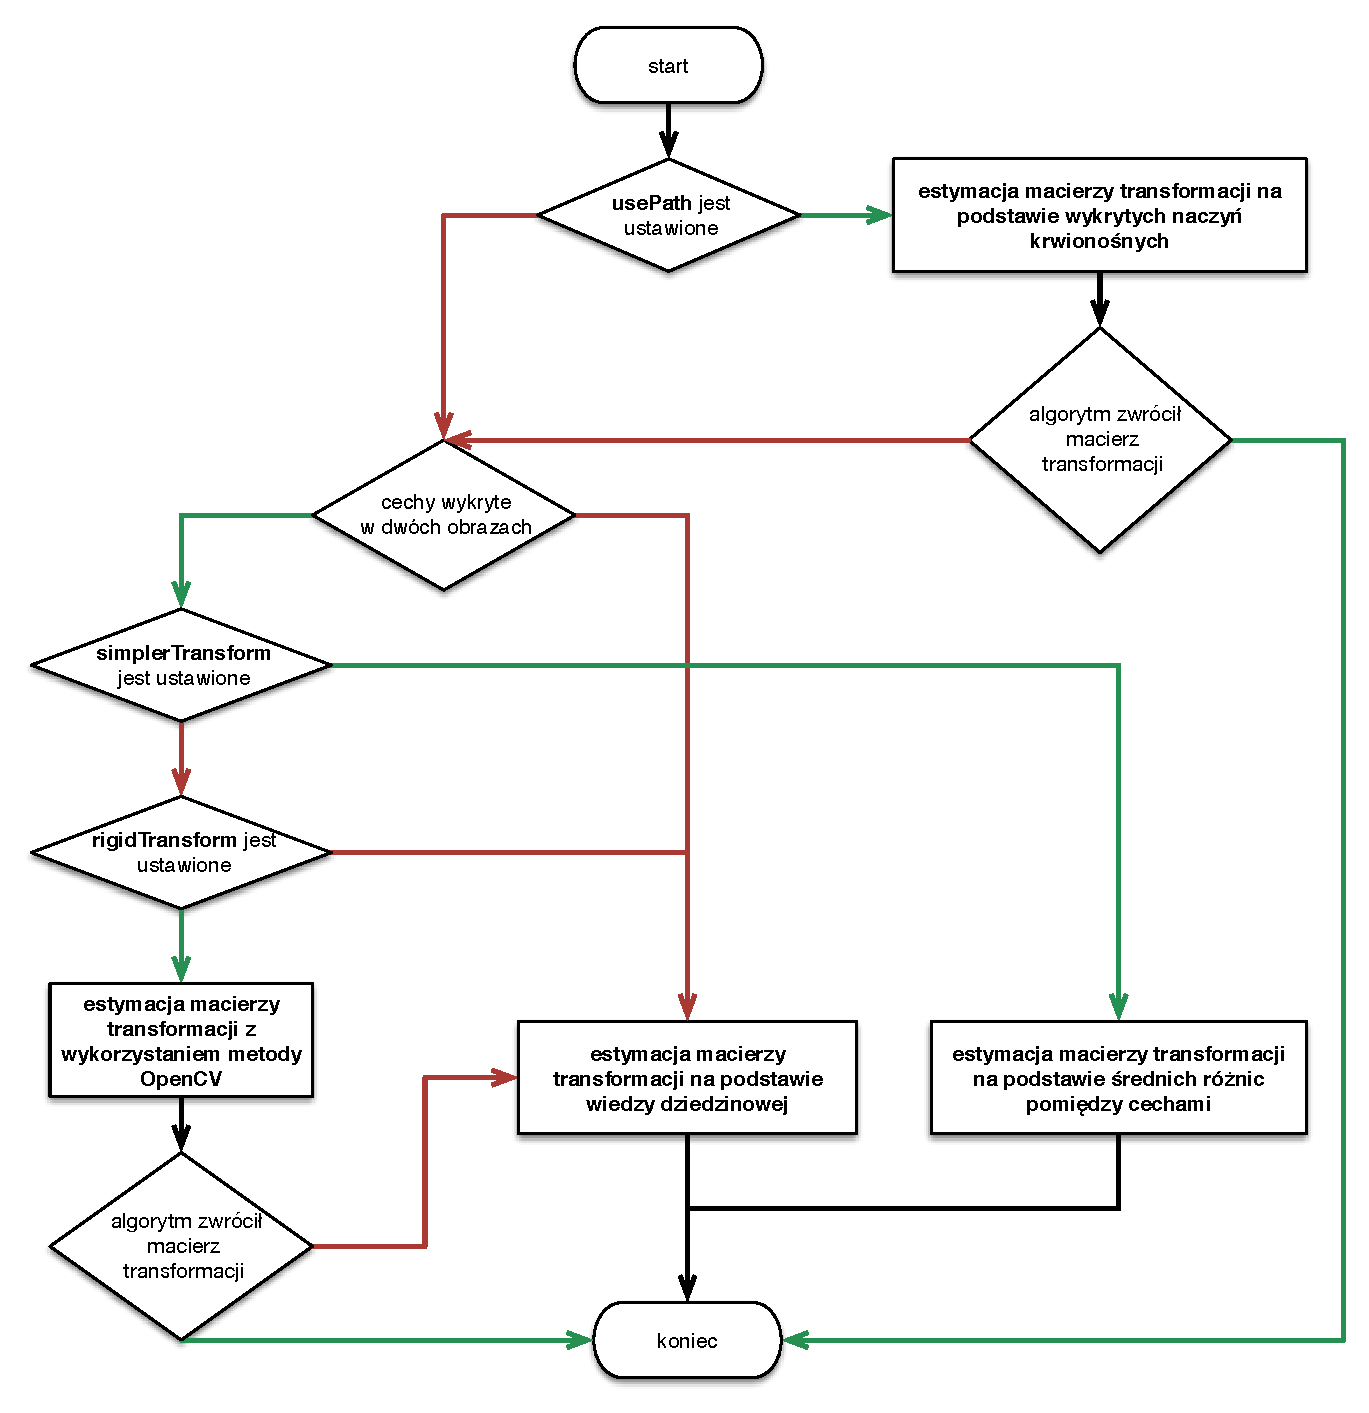
\includegraphics[width=\textwidth]{gfx/decision_model}
  \caption{Schemat blokowy wyjaśniający wybór metody estymacji macierzy transformacji w zależności od wewnętrznej zmiennej w programie (czerwone strzałki odpowiadają odpowiedzi `nie', a zielone strzałki odpowiadają odpowiedzi `tak').}
  \label{fig:proponowane_algorytmy:decision_model}
\end{figure}

\subsection{Proces decyzyjny}
\label{sec:proponowane_algorytmy:proces_decyzyjny}

Wybór użytej metody do estymacji macierzy transformacji jest głównie zdeterminowany przez trzy zmienne w programie \texttt{simplerTransform} (odpowiada metodzie z sekcji \ref{sec:proponowane_algorytmy:srednie_roznice}), \texttt{rigidTransform} (odpowiada metodzie z sekcji \ref{sec:proponowane_algorytmy:rigid}) i \texttt{usePaths} (opowiada metodzie z sekcji \ref{sec:proponowane_algorytmy:use_paths}). Algorytm samodzielnie tworzy różne kombinacje wartości zmiennych by na wyjściu uzyskać kilka mozaik. Dzięki temu mechanizmowi użytkownik ma możliwość wybrania najlepszego rezultatu. Rysunek \ref{fig:proponowane_algorytmy:decision_model} obrazuje proces wyboru metody w zależności od ustawionych parametrów.

\section{Globalna rejestracja kafelków}
\label{sec:proponowane_algorytmy:globalna_rejestracja}

Następnym krokiem tworzenia mozaiki jest decyzja, który kafelek rejestrować z którym i w jakiej kolejności. Proces rozpoczyna się od wybrania kafelka referencyjnego wobec którego wszystkie inne mozaiki będą transformowane. Zakładając, że mozaika składa się z $r$ wierszy i $c$ kolumn współrzędne kafelka referencyjnego $ref_x$ i $ref_y$ są wybierane na podstawie:
\begin{equation}
ref_x = \left \lfloor\frac{c - 1}{2}\right \rfloor
\label{eq:ref_x}
\end{equation}
\begin{equation}
ref_y = \left \lfloor\frac{r - 1}{2}\right \rfloor
\label{eq:ref_y}
\end{equation}
Mając wyznaczony kafelek referencyjny następnym krokiem jest ustalenie kolejności rejestracji pomiędzy kafelkami. Proces wyjaśniony jest na przykładzie na rysunku \ref{fig:proponowane_algorytmy:global_registration}.

\begin{figure}[H]
  \centering
  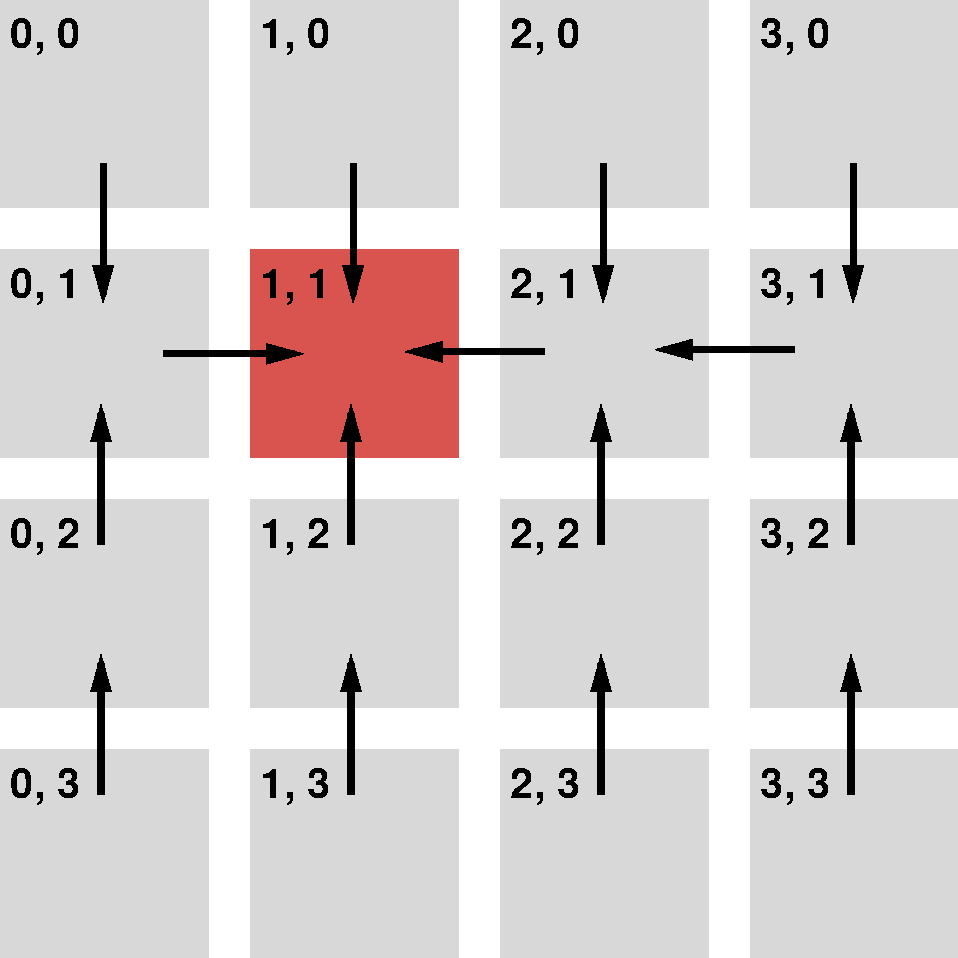
\includegraphics[width=5cm]{gfx/global_registration}
  \caption{Przykład mozaiki składającej się z 4 wierszy i 4 kolumn kafelków. Kafelek referencyjny wybrany zgodnie z wzorami \ref{eq:ref_x} i \ref{eq:ref_y} oznaczono kolorem czerwonym. Rejestracja kafelków rozpoczyna się od porównywania kafelków parami na lewo i prawo od kafelka referencyjnego. Następnie od każdego kafelka z wiersza kafelka referencyjnego kafelki są porównywane parami idąc w górę i dół. W lewym górnym rogu każdego kafelka jest zapisana jego współrzędna w mozaice.}
  \label{fig:proponowane_algorytmy:global_registration}
\end{figure}

Posługując się przykładem z rysunku \ref{fig:proponowane_algorytmy:global_registration} oraz oznaczając $T_{xy\rightarrow zw}$ jako macierz transformacji pomiędzy kafelkiem $I_{xy}$ o współrzędnych $x$ i $y$ i kafelkiem $I_{zw}$ o współrzędnych $z$ i $w$ macierz transformacji kafelka $I_{33}$ wygląda następująco:
\begin{equation}
T_{33\rightarrow 11} = T_{21\rightarrow 11}T_{31\rightarrow 21}T_{32\rightarrow 31}T_{33\rightarrow 32}
\end{equation}
\section{Łączenie kafelków}
\label{sec:proponowane_algorytmy:laczenie_kafelkow}

Ostatnim etapem w tworzeniu mozaiki jest wyświetlenie wszystkich kafelków po transformacji na wspólnej płaszczyźnie. Żeby mozaika spełniała wrażenie spójnej i jednolitej musi być zaimplementowany mechanizm, który będzie odpowiednio wybierał i ważył piksele w miejscach gdzie kafelki się nakładają. Wartość piksela finalnej mozaiki $f$ jest obliczana za pomocą wzoru:
\begin{equation}
f(p) = \frac{\sum_{n = 0}^{N - 1} w_n(p)f_n(p)}{\sum_{n = 0}^{N - 1} w_n(p)}
\end{equation}
Gdzie $N$ to liczba kafelków znajdujących się w miejscu piksela $f(p)$, $f_n(p)$ to wartość piksela $p$ w kafelku $n$, a $w_n(p)$ to waga piksela $p$ w kafelku $n$. Wagi pikseli są obliczane za pomocą \textbf{\textit{distance transform}}\footnote{\url{https://en.wikipedia.org/wiki/Distance_transform}}, której wartość to odległość do najbliższego piksela o wartości 0. \textit{Distance transform} jest zaimplementowane w OpenCV za pomocą funkcji \texttt{distanceTransform(...)} zwracającą obraz z obliczonymi wartościami dla całego obrazu. Rysunek \ref{fig:proponowane_algorytmy:dis} przedstawia wyjście funkcji na przykładowym obrazie.

\begin{figure}[H]
  \centering
  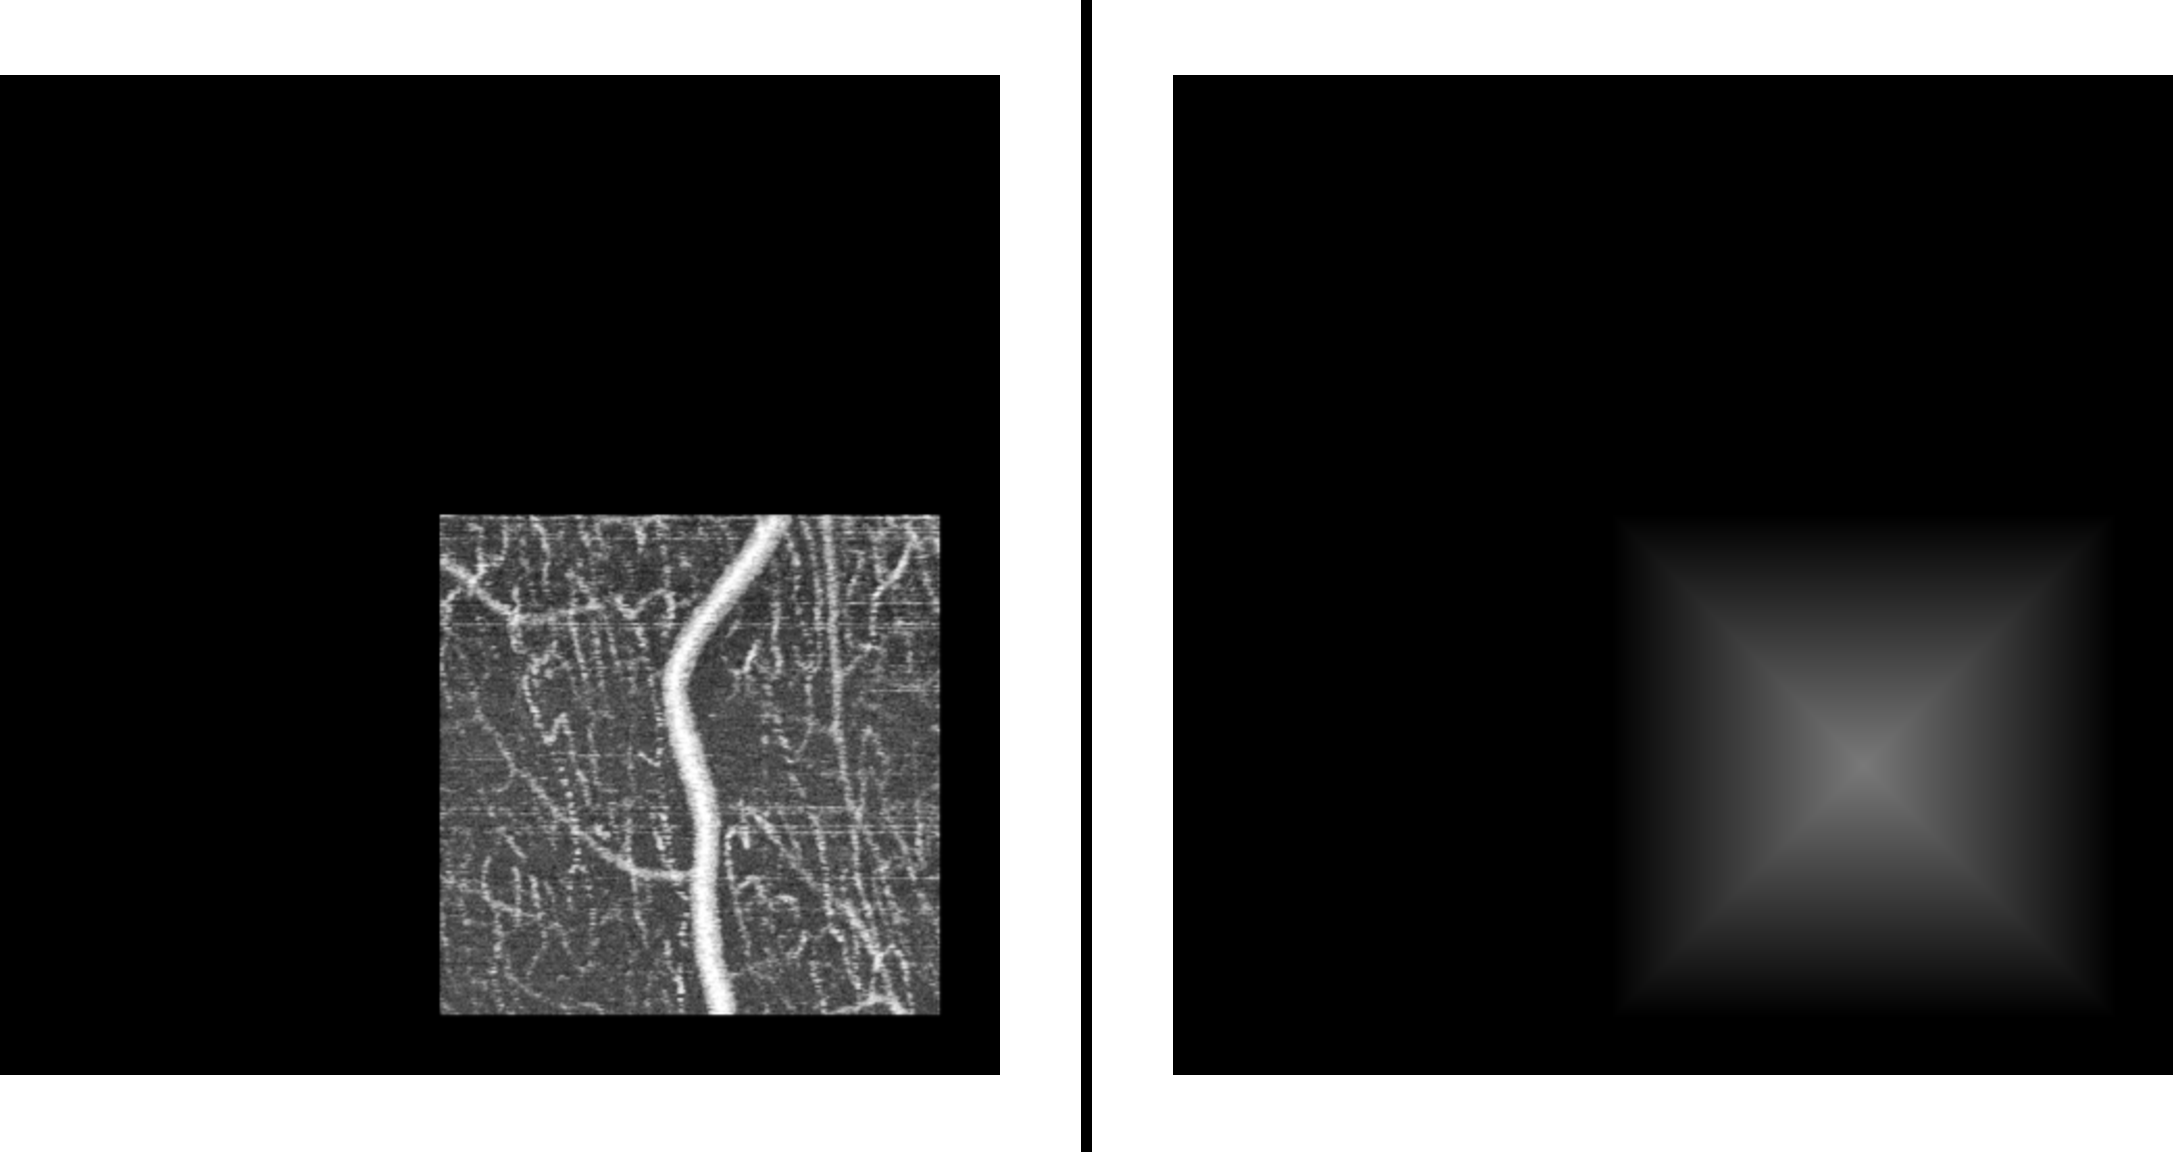
\includegraphics[width=10cm]{gfx/dis}
  \caption{\textbf{Lewy obraz:} Przykładowy kafelek po transformacji. \textbf{Prawy obraz:} Wyjście funkcji \texttt{distanceTransform(...)}.}
  \label{fig:proponowane_algorytmy:dis}
\end{figure}

Dzięki wykorzystaniu \textit{distance transform} piksele znajdujące się bliżej środka obrazu będą bardziej istotne w przeciwieństwie do pikseli znajdujących przy krawędziach obrazu. Rysunek \ref{fig:proponowane_algorytmy:blend} przedstawia przykładowe dwa kafelki z zaznaczonymi trzema punktami $p_1$, $p_2$ i $p_3$ w finalnej mozaice. Punkt $p_1$ nie należy do żadnego kafelka przez co jego wartość jest równa $0$, punkt $p_2$ należy do kafelka $f_2$ i jego wartość jest równa:
\begin{equation}
f(p_2) = \frac{d_{22}f_2(p_2)}{d_{22}}
\end{equation}
Gdzie $d_{nk}$ to wartość \textit{distance transform} piksela $p_n$ w obrazie $f_k$. Punkt $p_3$ należy do kafelka $f_2$ i $f_3$ i jego wartość jest równa:
\begin{equation}
f(p_3) = \frac{d_{32}f_2(p_3) + d_{31}f_1(p_3)}{d_{32} + d_{31}}
\end{equation}
\begin{figure}[H]
  \centering
  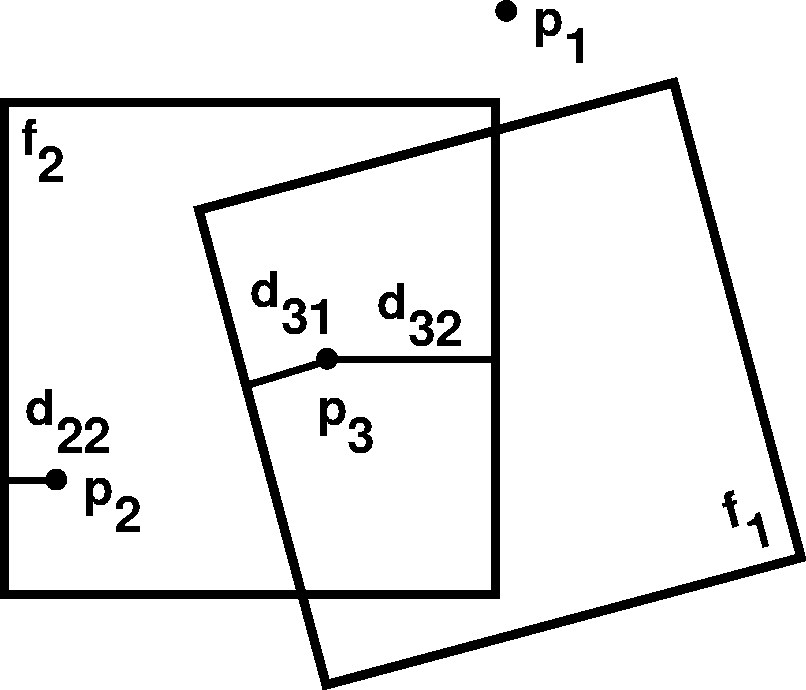
\includegraphics[width=6cm]{gfx/blend}
  \caption{Przykładowy schemat łączenia dwóch kafelków $f_1$ i $f_2$ z zaznaczonymi punktami $f_n$ oraz wartościami \textit{distance transform} $d_nk$.}
  \label{fig:proponowane_algorytmy:blend}
\end{figure}

Rysunek \ref{fig:proponowane_algorytmy:blend_eff} przedstawia wynik łączenia kafelków niniejszą metodą na przykładowej mozaice.

\begin{figure}[H]
  \centering
  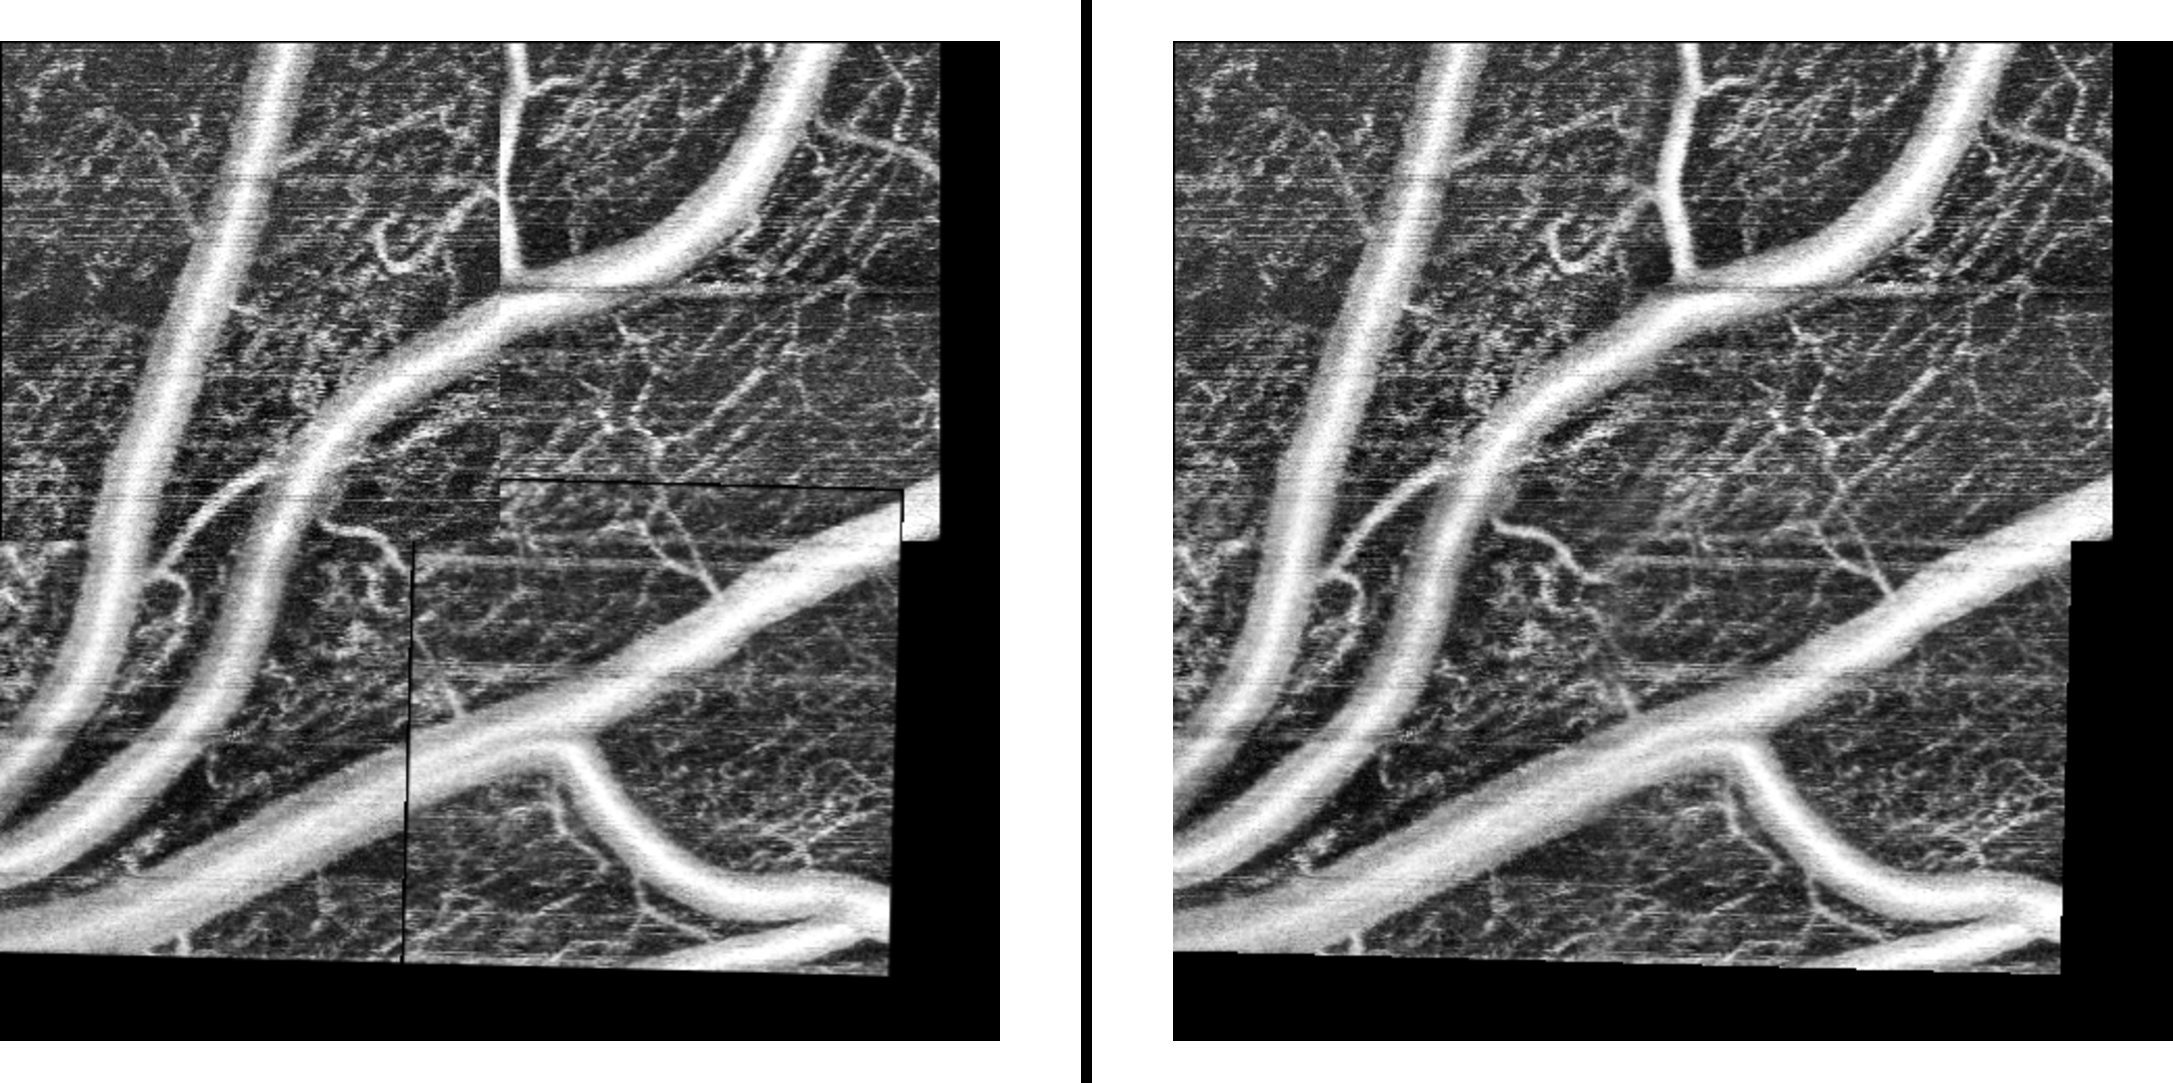
\includegraphics[width=8cm]{gfx/blend_eff}
  \caption{\textbf{Lewy obraz:} Mozaika stworzona bez wykorzystania łączenia. \textbf{Prawy obraz:} ozaika stworzona z wykorzystaniem łączenia.}
  \label{fig:proponowane_algorytmy:blend_eff}
\end{figure}
